\documentclass[10pt, a4paper]{article}
\usepackage[utf8]{inputenc}
\usepackage[top=0.7in, bottom=0.7in, left=0.75in, right=0.75in]{geometry}
\usepackage{graphicx}
\usepackage{amsmath}
\usepackage{amssymb}
\usepackage{booktabs}
\usepackage{hyperref}
\usepackage{xcolor}
\usepackage{caption}
\usepackage{float}
\usepackage{array}

\graphicspath{{"Question Network/"}{"Extreme Bipartite Network/extreme_plots/"}{"Student Network/student_plots/"}}

\definecolor{techblue}{HTML}{1F77B4}
\definecolor{eduorange}{HTML}{FF7F0E}
\definecolor{socgreen}{HTML}{2CA02C}
\definecolor{envpurple}{HTML}{9467BD}
\definecolor{darkink}{HTML}{0B0B0B}

\hypersetup{
    colorlinks=true,
    linkcolor=techblue,
    urlcolor=techblue,
    citecolor=socgreen
}

\title{\vspace{-1.8em}\textbf{Opinion Network Formation: Multi-Scale Analysis Across Student Projections, Bipartite Extremes, and Item Correlations}\vspace{-0.5em}}
\author{
    \textbf{Team Name:} \textit{[Insert Team Name Here]} \quad $\vert$ \quad \textbf{Course:} Distributed Systems \& Complex Networks (DPCN) \\
    \textbf{Team Members:} Mayank Kar, Tanush Garg, Amish Goyal \quad $\vert$ \quad \textbf{Institution:} IIIT Hyderabad \\
    \textbf{GitHub Repository:} \url{https://github.com/your-username/DPCN_ass1} \quad $\vert$ \quad
    \textbf{Interactive Dashboard:} \url{https://your-username.github.io/DPCN_ass1/}
}
\date{\vspace{-0.6em}\textbf{Assignment 1 Report} \quad $\vert$ \quad \textbf{Submission Date:} September 20, 2026\vspace{-0.9em}}

\begin{document}
\maketitle

\begin{abstract}
\small
We investigate the latent opinion landscape of a university cohort ($N=91$ active respondents, $M=60$ Likert statements) across Technology (T), Education (E), Society \& Ethics (S), and Environment (V). To cut through severe ambient positivity bias ($79.8\%$ positive responses), we analyze the belief architecture across three complementary network paradigms: (1)~\textbf{Student--Student Opinion Network} (chance-adjusted similarity, small-world cohesion, and topic-specific alignment), (2)~\textbf{Bipartite Extremes Network} (filtering for high conviction $\tau \in \{1, 5\}$, proving overdispersed non-scale-free degree distribution, $K_{60}$ projection, and Molloy--Reed percolation $\kappa = 59 \gg 2$), and (3)~\textbf{Question--Question Correlation Network} (Spearman $\rho > 0.35$, isolating ideological anchors, cross-domain bridges, and 6 modular belief communities with assortativity $r = 0.3044$). All interactive D3 visualizers and complete high-resolution plot galleries are hosted on our public web portal.
\end{abstract}

\vspace{-0.6em}
\hrule
\vspace{0.6em}

%% ====================================================================
\section{Dataset Documentation: Interpretation and Preparation}
%% ====================================================================

\subsection{Survey Design and Thematic Categories}
The dataset comprises $N = 96$ raw student submissions across $M = 60$ normative propositions divided equally into four thematic domains (15 questions each):
\begin{itemize}
    \setlength{\itemsep}{0pt}
    \item \textbf{Technology (\texttt{T01}--\texttt{T15}):} Evaluates artificial intelligence ethics, algorithmic governance, digital surveillance, and workforce automation.
    \item \textbf{Education (\texttt{E01}--\texttt{E15}):} Probes higher-education pedagogical models, curriculum modernization, experiential learning, and generative AI adoption.
    \item \textbf{Society \& Ethics (\texttt{S01}--\texttt{S15}):} Examines campus diversity and inclusion, institutional equity, corporate accountability, and digital literacy.
    \item \textbf{Environment (\texttt{V01}--\texttt{V15}):} Focuses on biodiversity preservation, renewable energy investment, campus green practices, and intergenerational climate justice.
\end{itemize}

\subsection{Likert Scale Encodings and Missing Data Handling}
Survey responses were collected on a standard 5-point Likert scale. We utilize a centered ordinal integer encoding $[-2, +2]$ (as well as discrete $[1, 5]$):
\[
\text{Strongly Disagree } (-2 / 1), \quad \text{Disagree } (-1 / 2), \quad \text{Neutral } (0 / 3), \quad \text{Agree } (+1 / 4), \quad \text{Strongly Agree } (+2 / 5)
\]
Centering at zero preserves polarity, ensuring positive values reflect agreement, negative values reflect disagreement, and zero represents neutrality. Out of 96 raw respondents, 5 submissions had zero answers across all 60 statements and were removed, yielding an active cohort of $N = 91$ students. Missing cells (242 entries across skipped items or ``No Comments'') were treated via pairwise complete observations.

\subsection{The Prevalence of Positivity Bias}
An empirical tally reveals heavy positive skew: 43.1\% Strongly Agree, 36.7\% Agree, 13.1\% Neutral, 4.9\% Disagree, and 2.1\% Strongly Disagree. With \textbf{79.8\% of responses in agreement}, naive similarity metrics inevitably produce trivial, saturated complete graphs. The three network pipelines below apply principled mathematical filters to uncover genuine structural co-variation.

%% ====================================================================
\section{Pipeline Followed: Three Complementary Network Formulations}
%% ====================================================================

\begin{table}[H]
\centering
\small
\caption{Methodological Architecture of the Three Network Formulations}
\label{tab:pipeline_summary}
\begin{tabular}{p{2.6cm} p{4.3cm} p{4.6cm} p{4.3cm}}
\toprule
\textbf{Dimension} & \textbf{1. Student--Student Network} & \textbf{2. Bipartite Extremes Network} & \textbf{3. Question--Question Network} \\
\midrule
\textbf{Node Sets} & Students ($N=91$) & Students ($U=89$), Questions ($V=60$) & Questions ($V=60$) \\
\textbf{Filtering Metric} & Chance-adjusted score $>0$; top-2 backbone & Absolute extremes $\tau \in \{1, 5\}$; drop $\{2, 3, 4\}$ & Spearman rank correlation $\rho > 0.35$ \\
\textbf{Edge Semantics} & $w = \text{Score} - \text{Chance}$; $d = 1/w$ & Unweighted bipartite; $w = |U_{ij}|$ in projection & Affinity $w = \rho$; Metric distance $d = 1/\rho$ \\
\textbf{Core Objective} & Social cohesion \& student typologies & Ideological passion \& percolation & Ideological anchors \& bridges \\
\bottomrule
\end{tabular}
\end{table}

\subsection{Student--Student Network Pipeline}
To correct for ambient consensus, the agreement between students $i$ and $j$ is adjusted by subtracting the expected agreement under independent random sampling: $S_{ij} = \sum_{k} s(x_{ik}, x_{jk}) - \mathbb{E}[s(x_{\cdot k}, x_{\cdot k})]$. Edges exist only when mutual agreement exceeds chance. A top-2 sparsified backbone is extracted to map irreducible social ties.

\subsection{Bipartite Extremes Pipeline}
Isolates intense conviction via the filter $f(r) = 1 \iff r \in \{1, 5\}$. Moderate and neutral responses are discarded, retaining 2,362 extreme edges across 89 students and 60 questions. Degree distributions are fitted to test scale-free vs. Poisson behavior, and the network is projected onto $V$ for Molloy--Reed percolation evaluation.

\subsection{Question--Question Correlation Pipeline}
Pairwise monotonic relationships $\rho_{ij}$ are evaluated for all $\binom{60}{2} = 1770$ statement pairs using Spearman rank correlation. Suprathreshold edges ($\rho > 0.35$) establish an undirected graph $G = (V, E)$, upon which power-iteration Eigenvector centrality (anchors), geodesic Betweenness centrality (bridges), Louvain modularity, and category attribute assortativity are computed.

%% ====================================================================
\section{Analysis and Visualizations: Graphical Representations \& Key Metrics}
%% ====================================================================

\textit{Note: All figures below are representative multi-panel summaries. Complete high-resolution 300 DPI exports, interactive HTML visualizers, and raw data are hosted on our public portal at \url{https://your-username.github.io/DPCN_ass1/}.}

\subsection{Student--Student Opinion Network: Cohesion, Topology, and Alignment}
The chance-adjusted student network forms a connected macro-component exhibiting pronounced \textbf{small-world characteristics}: high local clustering ($\langle C \rangle = 0.712$, $1.52\times$ higher than an equivalent random graph) and short geodesic paths ($\langle L \rangle = 1.642$), yielding a small-world coefficient $\sigma \approx 1.52$ (full) and $\sigma \approx 5.74$ on the top-2 backbone.

\begin{figure}[H]
    \centering
    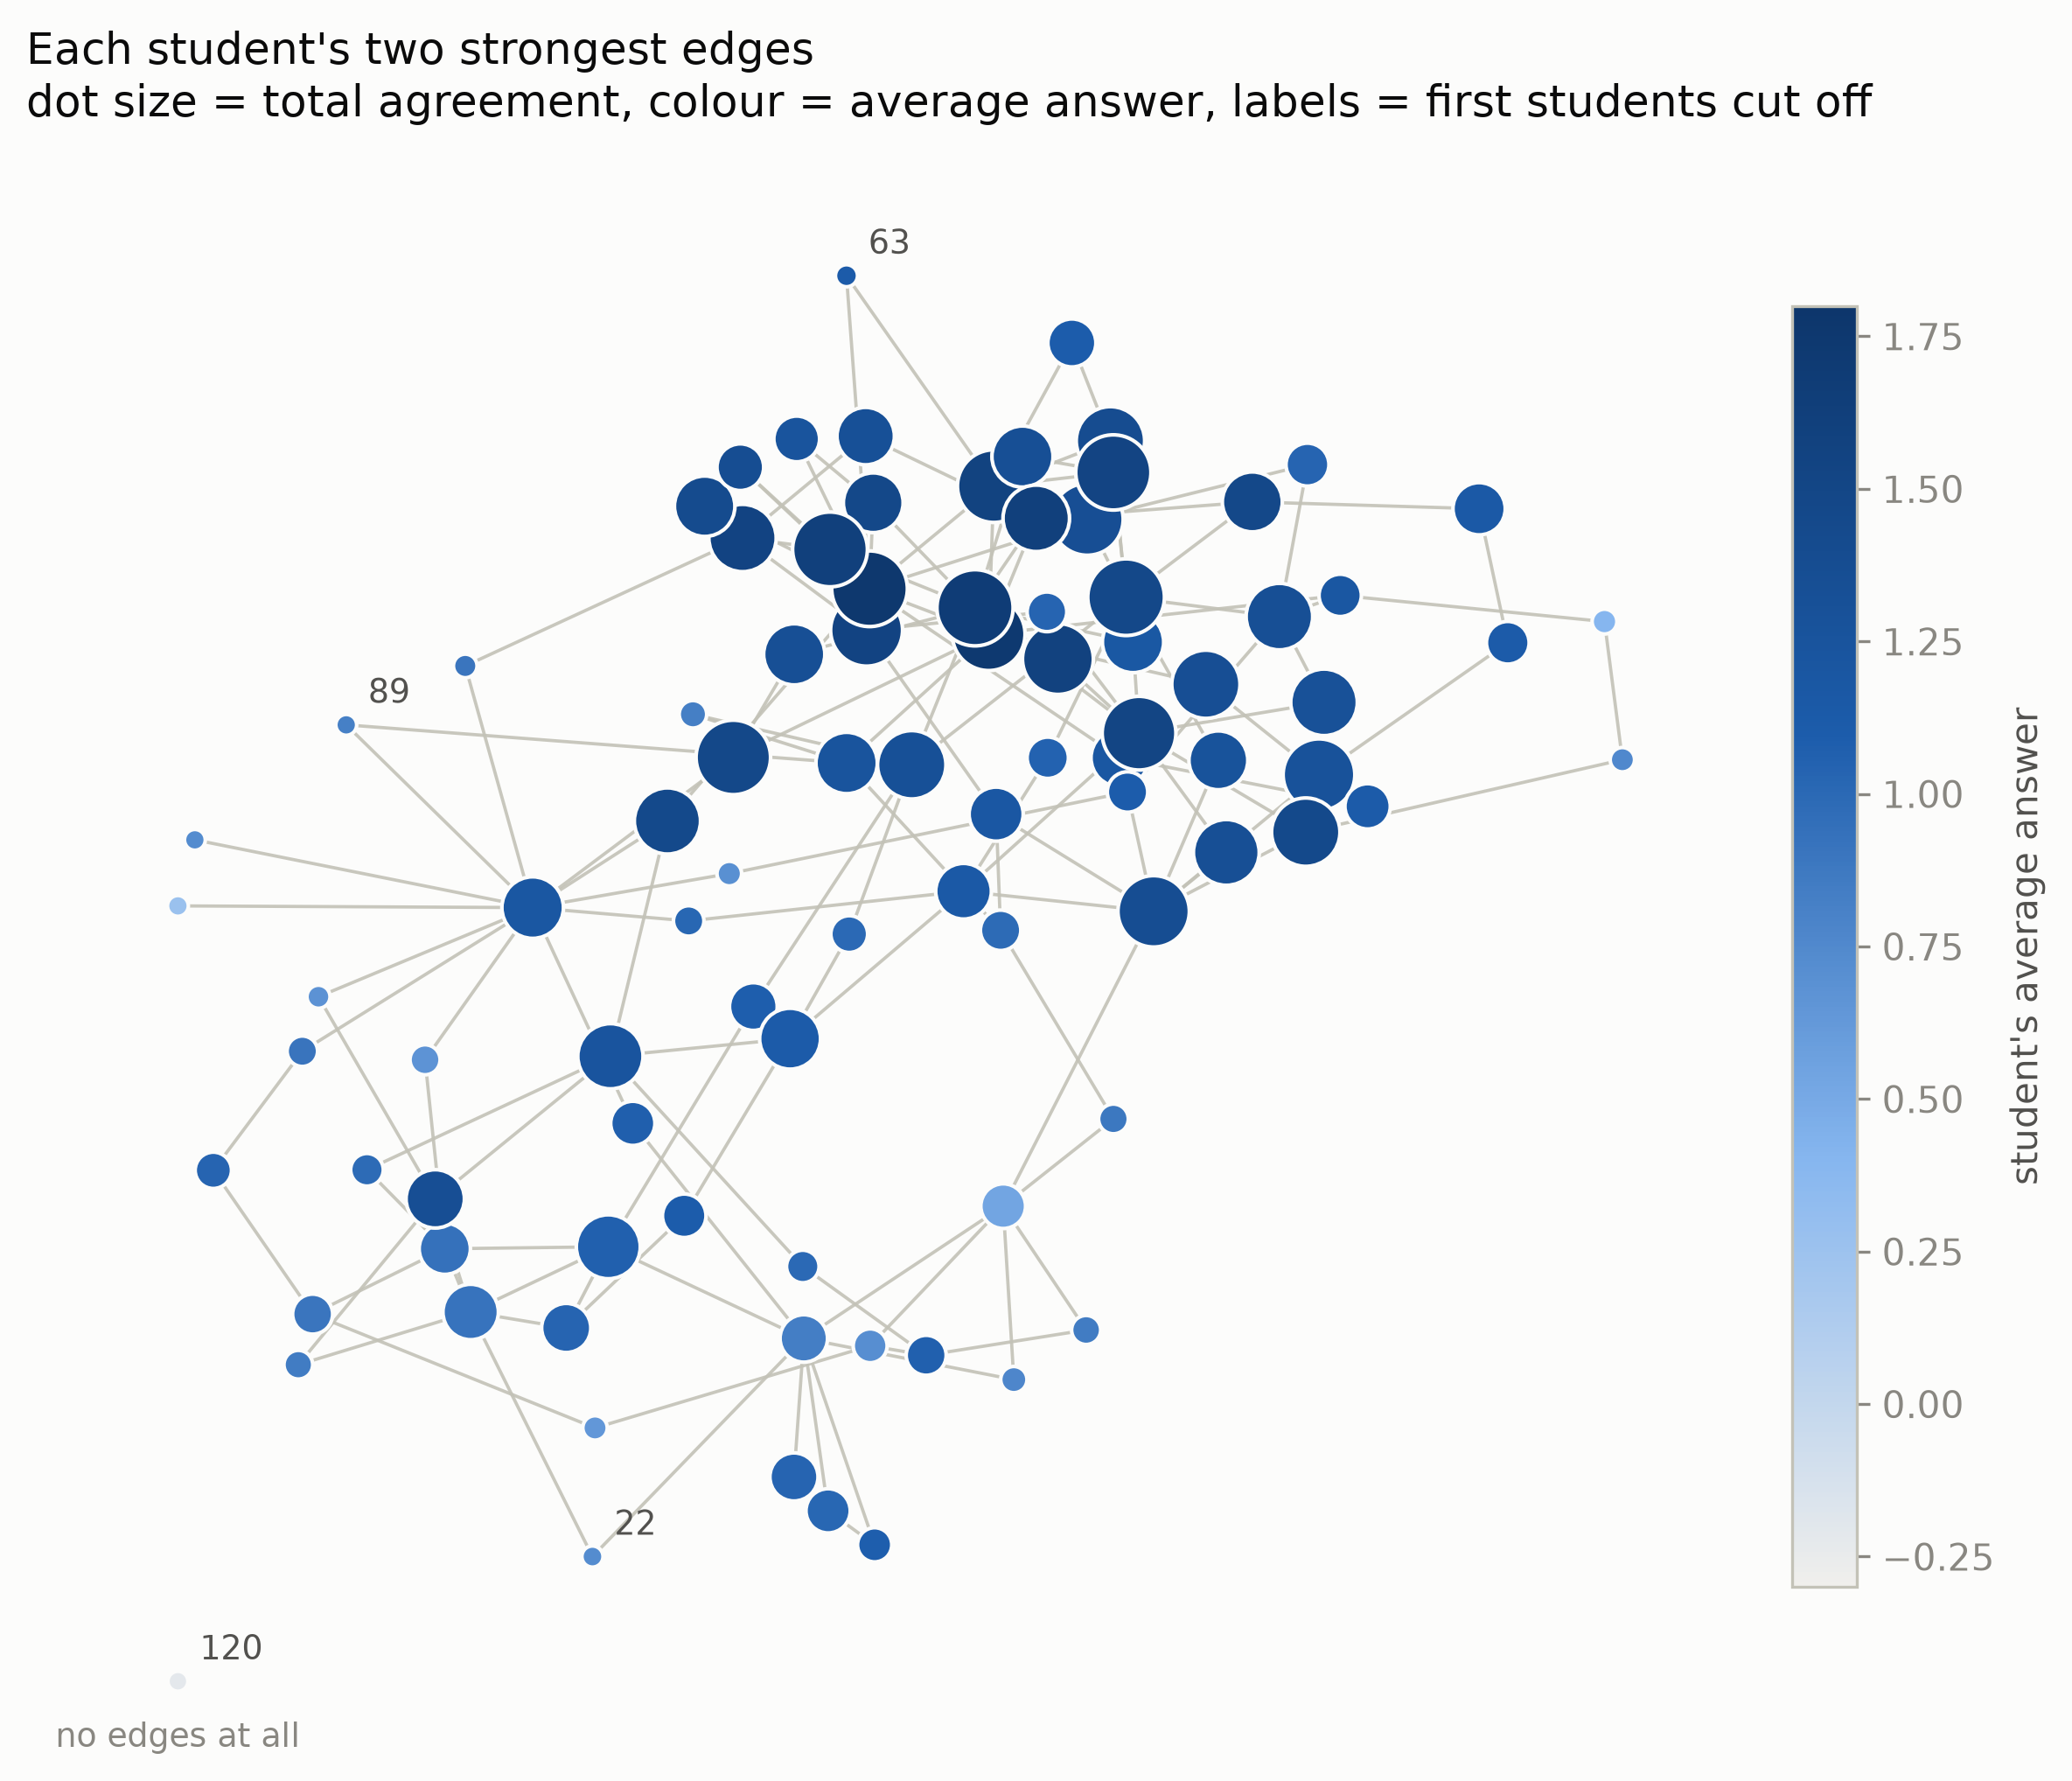
\includegraphics[width=0.48\textwidth]{Student Network/student_plots/network_drawing.png} \hfill
    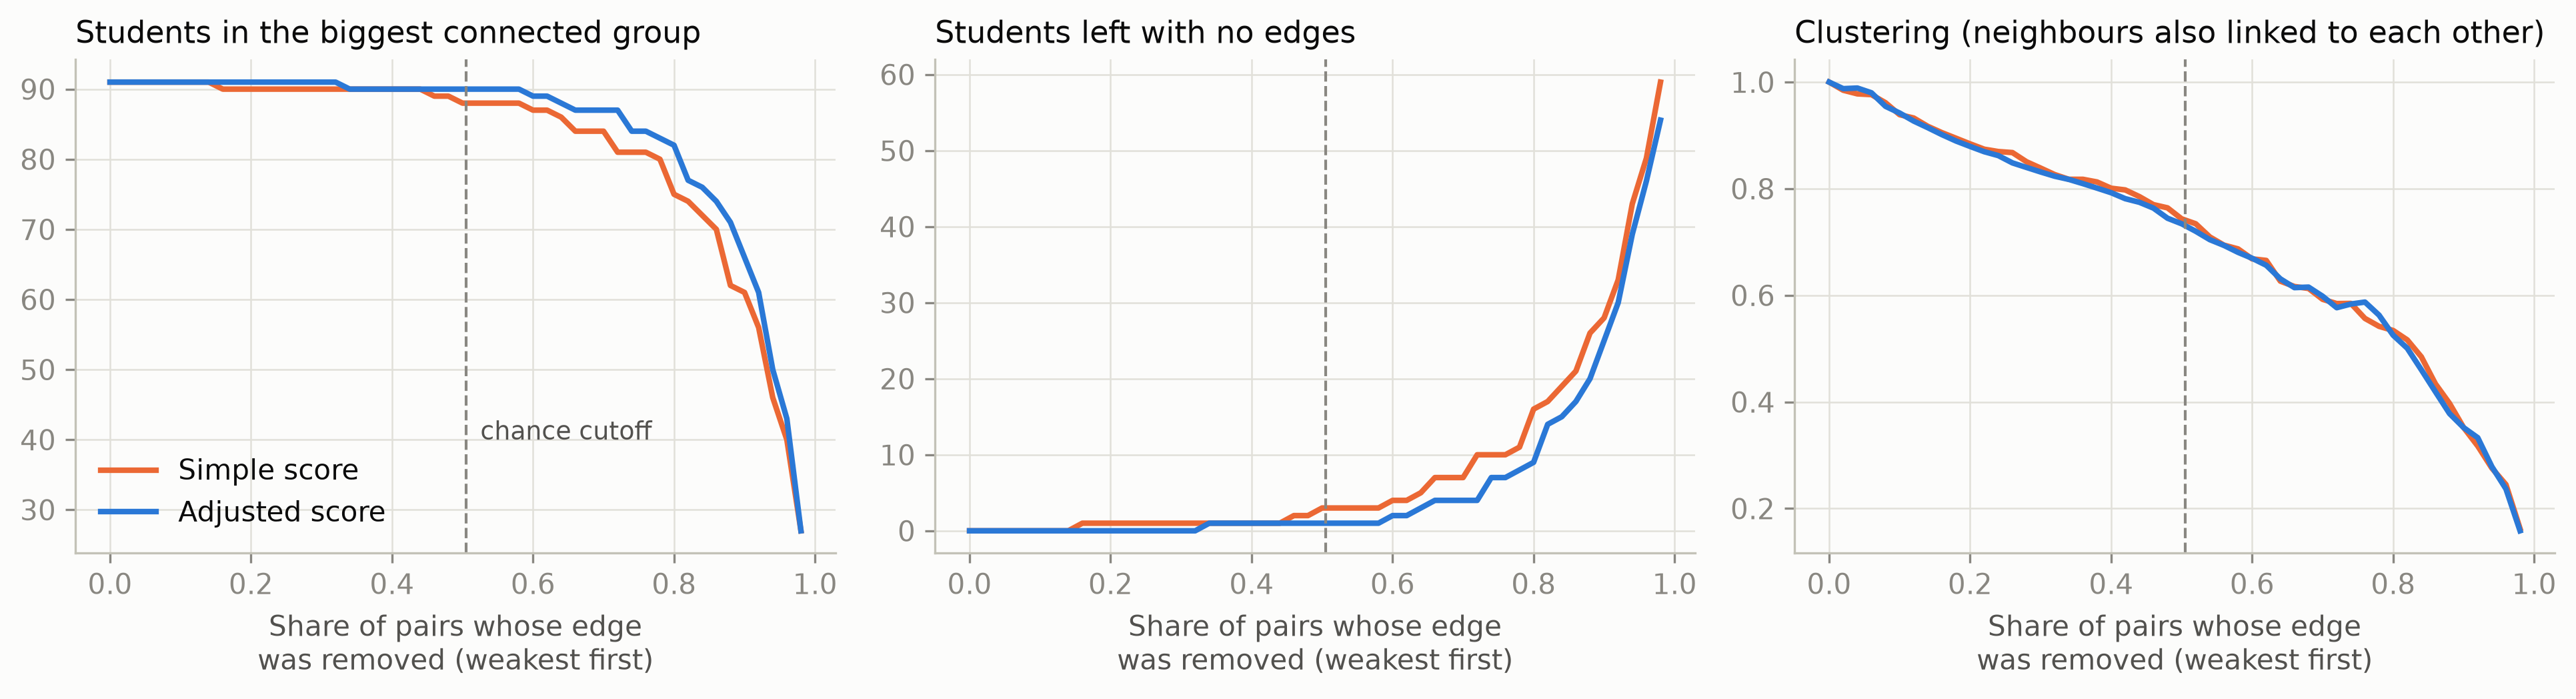
\includegraphics[width=0.48\textwidth]{Student Network/student_plots/threshold_sweep.png}
    \caption{\textbf{Student Network Topology and Sparsification:} (Left) Chance-adjusted student network layout (node color indicates degree; edge opacity reflects agreement strength beyond chance). (Right) Threshold sweep showing gradual percolation degradation without sudden fragmentation.}
    \label{fig:student_topo_sweep}
\end{figure}

\begin{figure}[H]
    \centering
    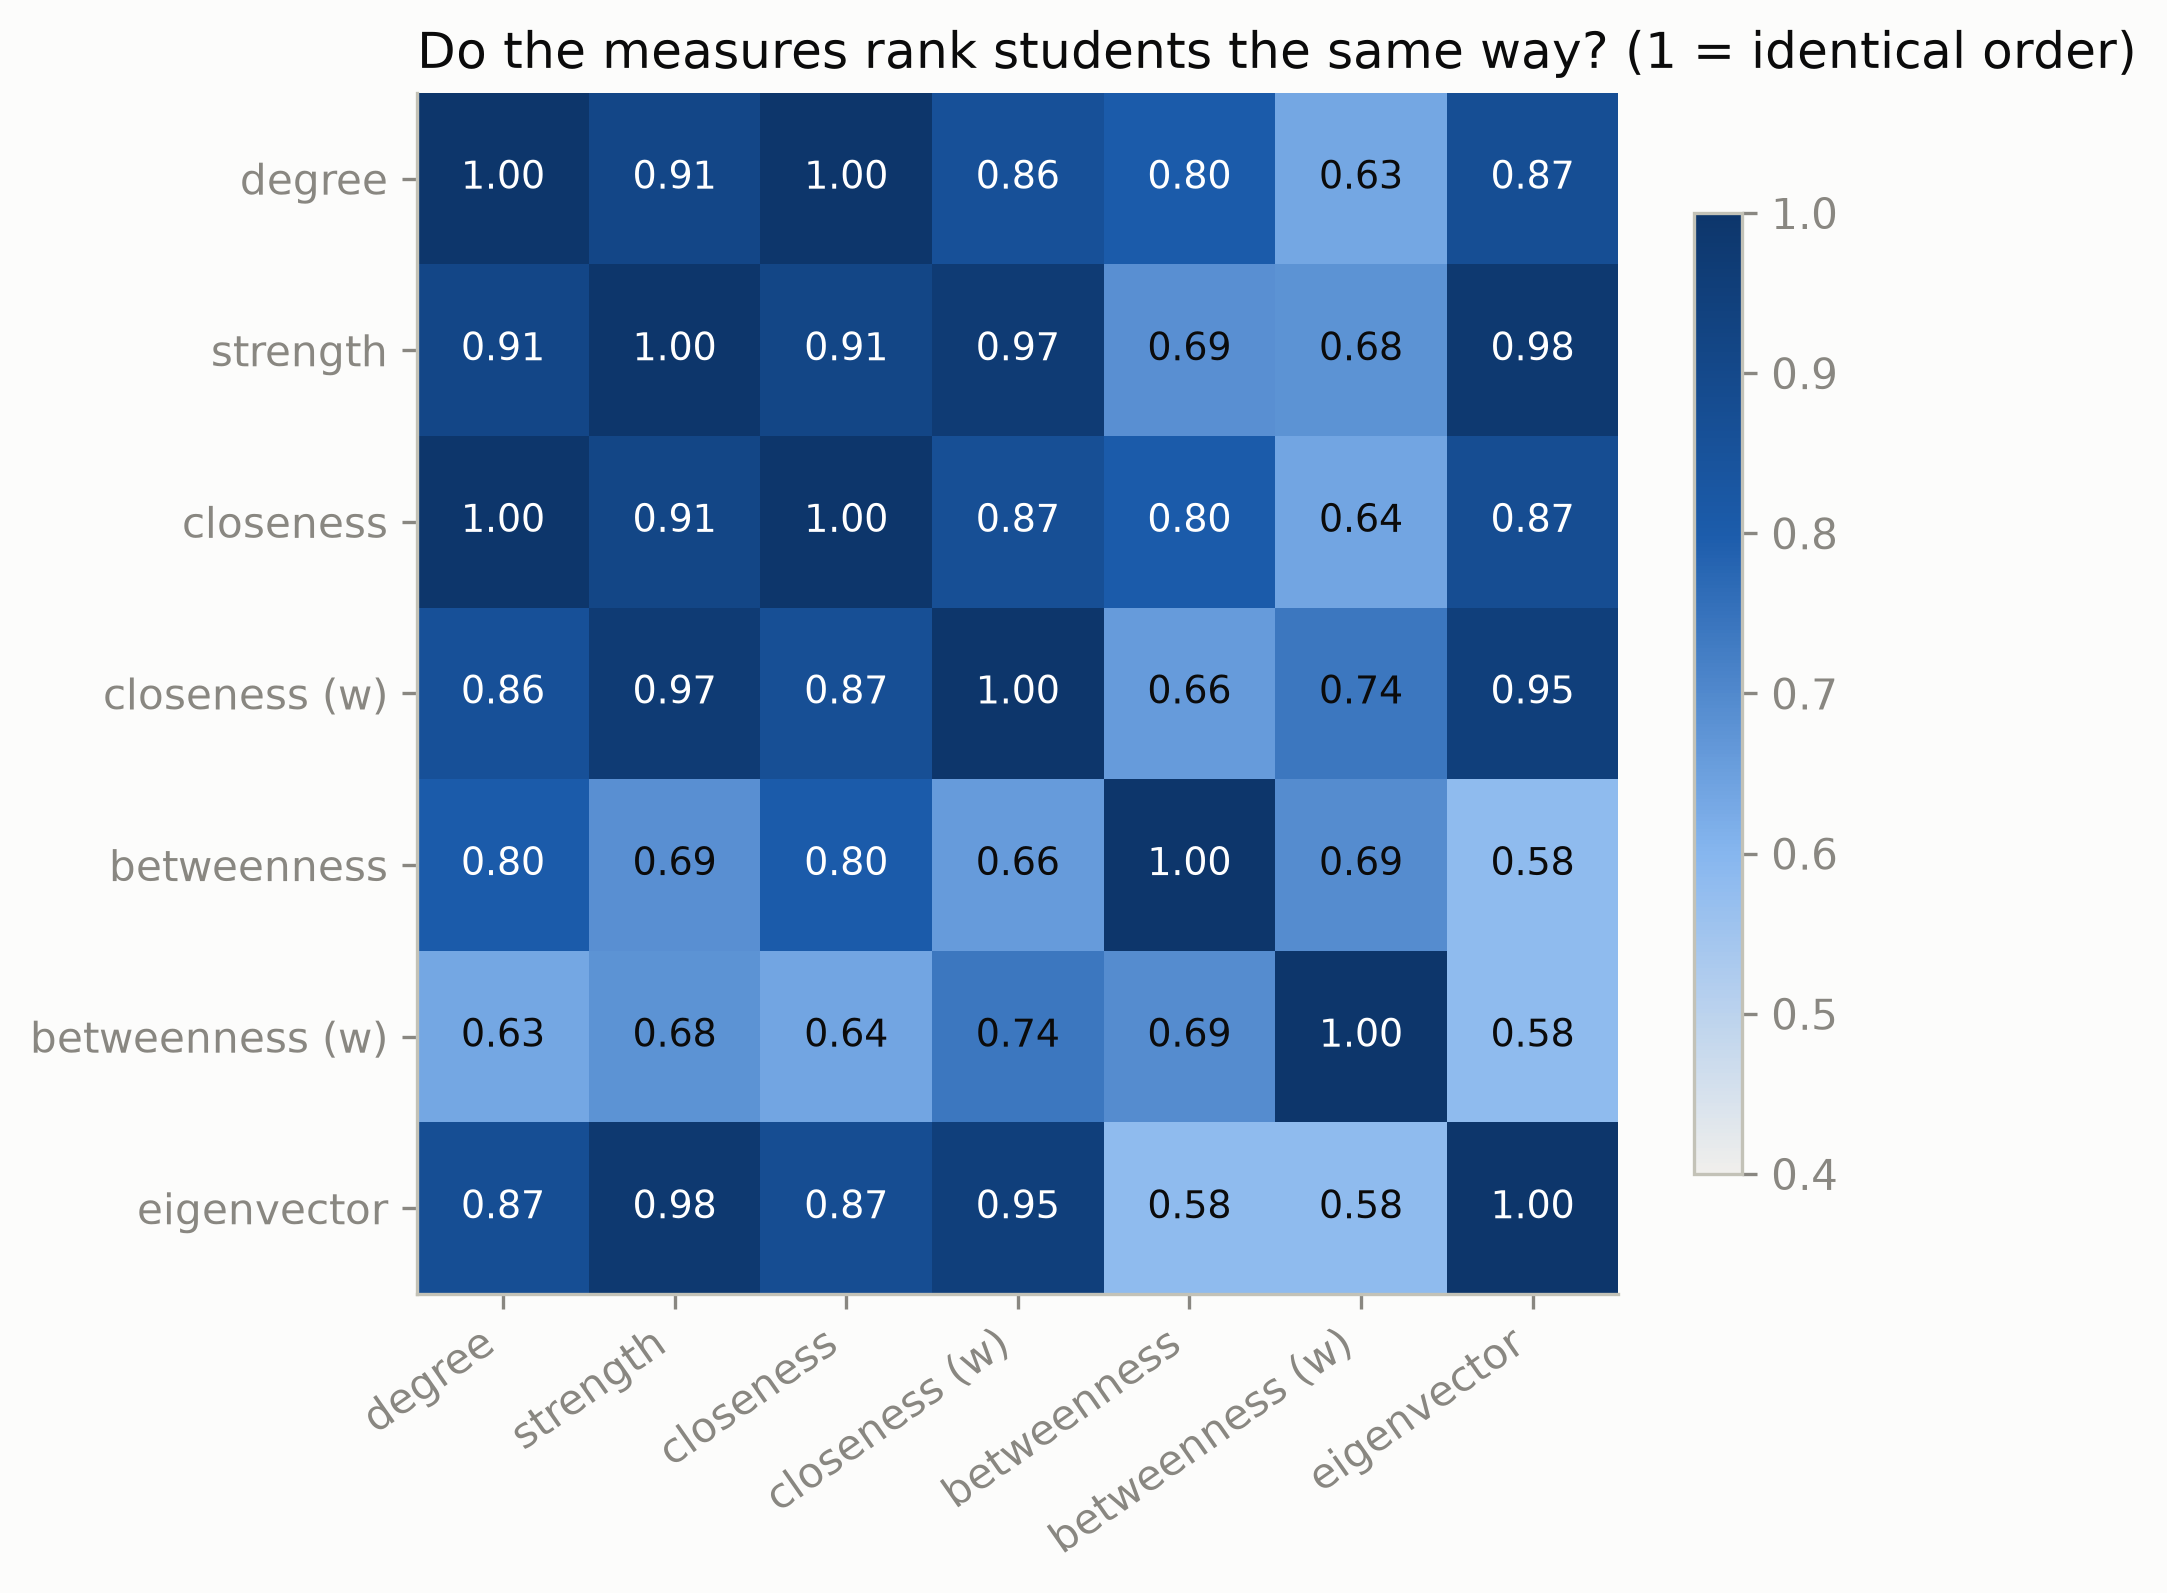
\includegraphics[width=0.48\textwidth]{Student Network/student_plots/centrality_correlations.png} \hfill
    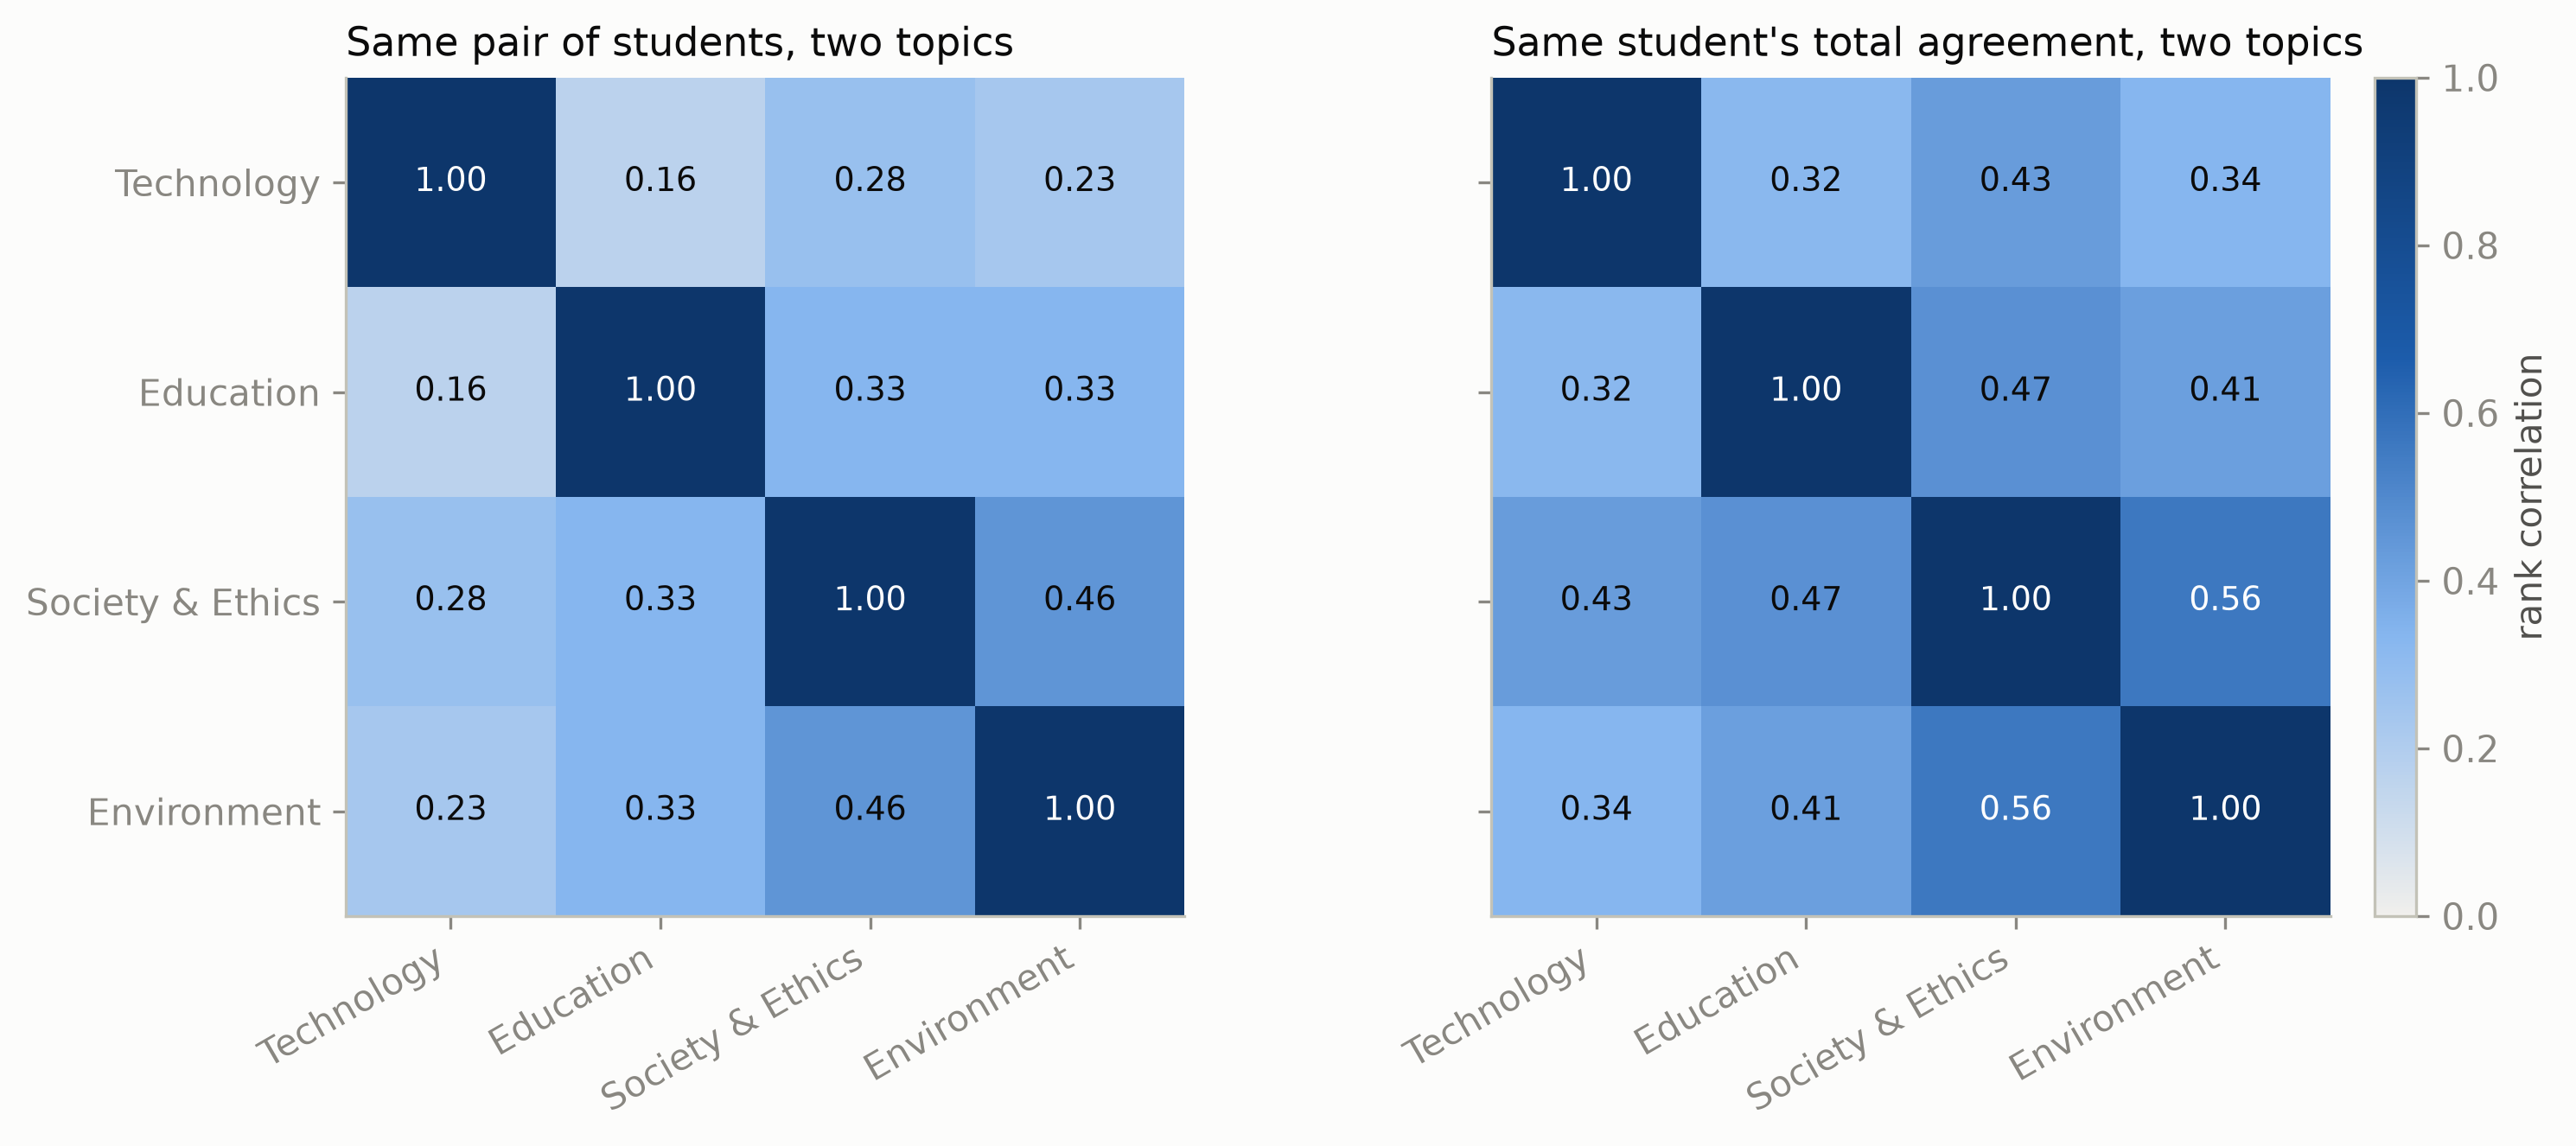
\includegraphics[width=0.48\textwidth]{Student Network/student_plots/topic_comparison.png}
    \caption{\textbf{Centrality Metrics and Cross-Topic Alignment:} (Left) Spearman rank correlation across student centralities. (Right) Cross-topic concordance: Society and Environment correlate strongly ($r = 0.46$), while Technology and Education align weakly ($r = 0.16$).}
    \label{fig:student_metrics_topic}
\end{figure}

\begin{table}[H]
\centering
\small
\caption{Student Network Topological Metrics Across Network Configurations}
\label{tab:student_small_world}
\begin{tabular}{lcccc}
\toprule
\textbf{Configuration} & \textbf{Clustering $\langle C \rangle$} & \textbf{Path Length $\langle L \rangle$} & \textbf{Degree Variance $\sigma^2_k$} & \textbf{Small-World $\sigma$} \\
\midrule
Full Thresholded Graph ($S_{ij} > 0$) & $0.712$ & $1.642$ & $142.3$ & $\mathbf{1.52}$ \\
Top-2 Backbone Graph                  & $0.485$ & $3.120$ & $4.18$  & $\mathbf{5.74}$ \\
Erd\H{o}s--R\'enyi (ER) Null Model    & $0.468$ & $1.625$ & $21.2$  & $1.00$ \\
\bottomrule
\end{tabular}
\end{table}

\textbf{Student Typologies:} Centrality analysis uncovers two distinct influential groups: (1)~\textbf{Emphatic consensus students} (41, 67, 94, 110) dominate Strength and Eigenvector centrality by registering strong agreement across almost all items; (2)~\textbf{Typical moderate students} (38, 52, 53, 99) maximize Degree and Closeness by bridging between moderate and emphatic peers. Peripheral students (120, 119, 125) hold averages well below neutral.

\subsection{Bipartite Extremes Network: Degree Distributions, Percolation, and Projection}
Filtering strictly for extreme convictions ($\tau \in \{1, 5\}$) yields an active bipartite graph $B = (U, V, E)$ with $|U| = 89$ students, $|V| = 60$ questions, and $|E| = 2{,}362$ edges (density $\delta = 0.4423$).

\begin{figure}[H]
    \centering
    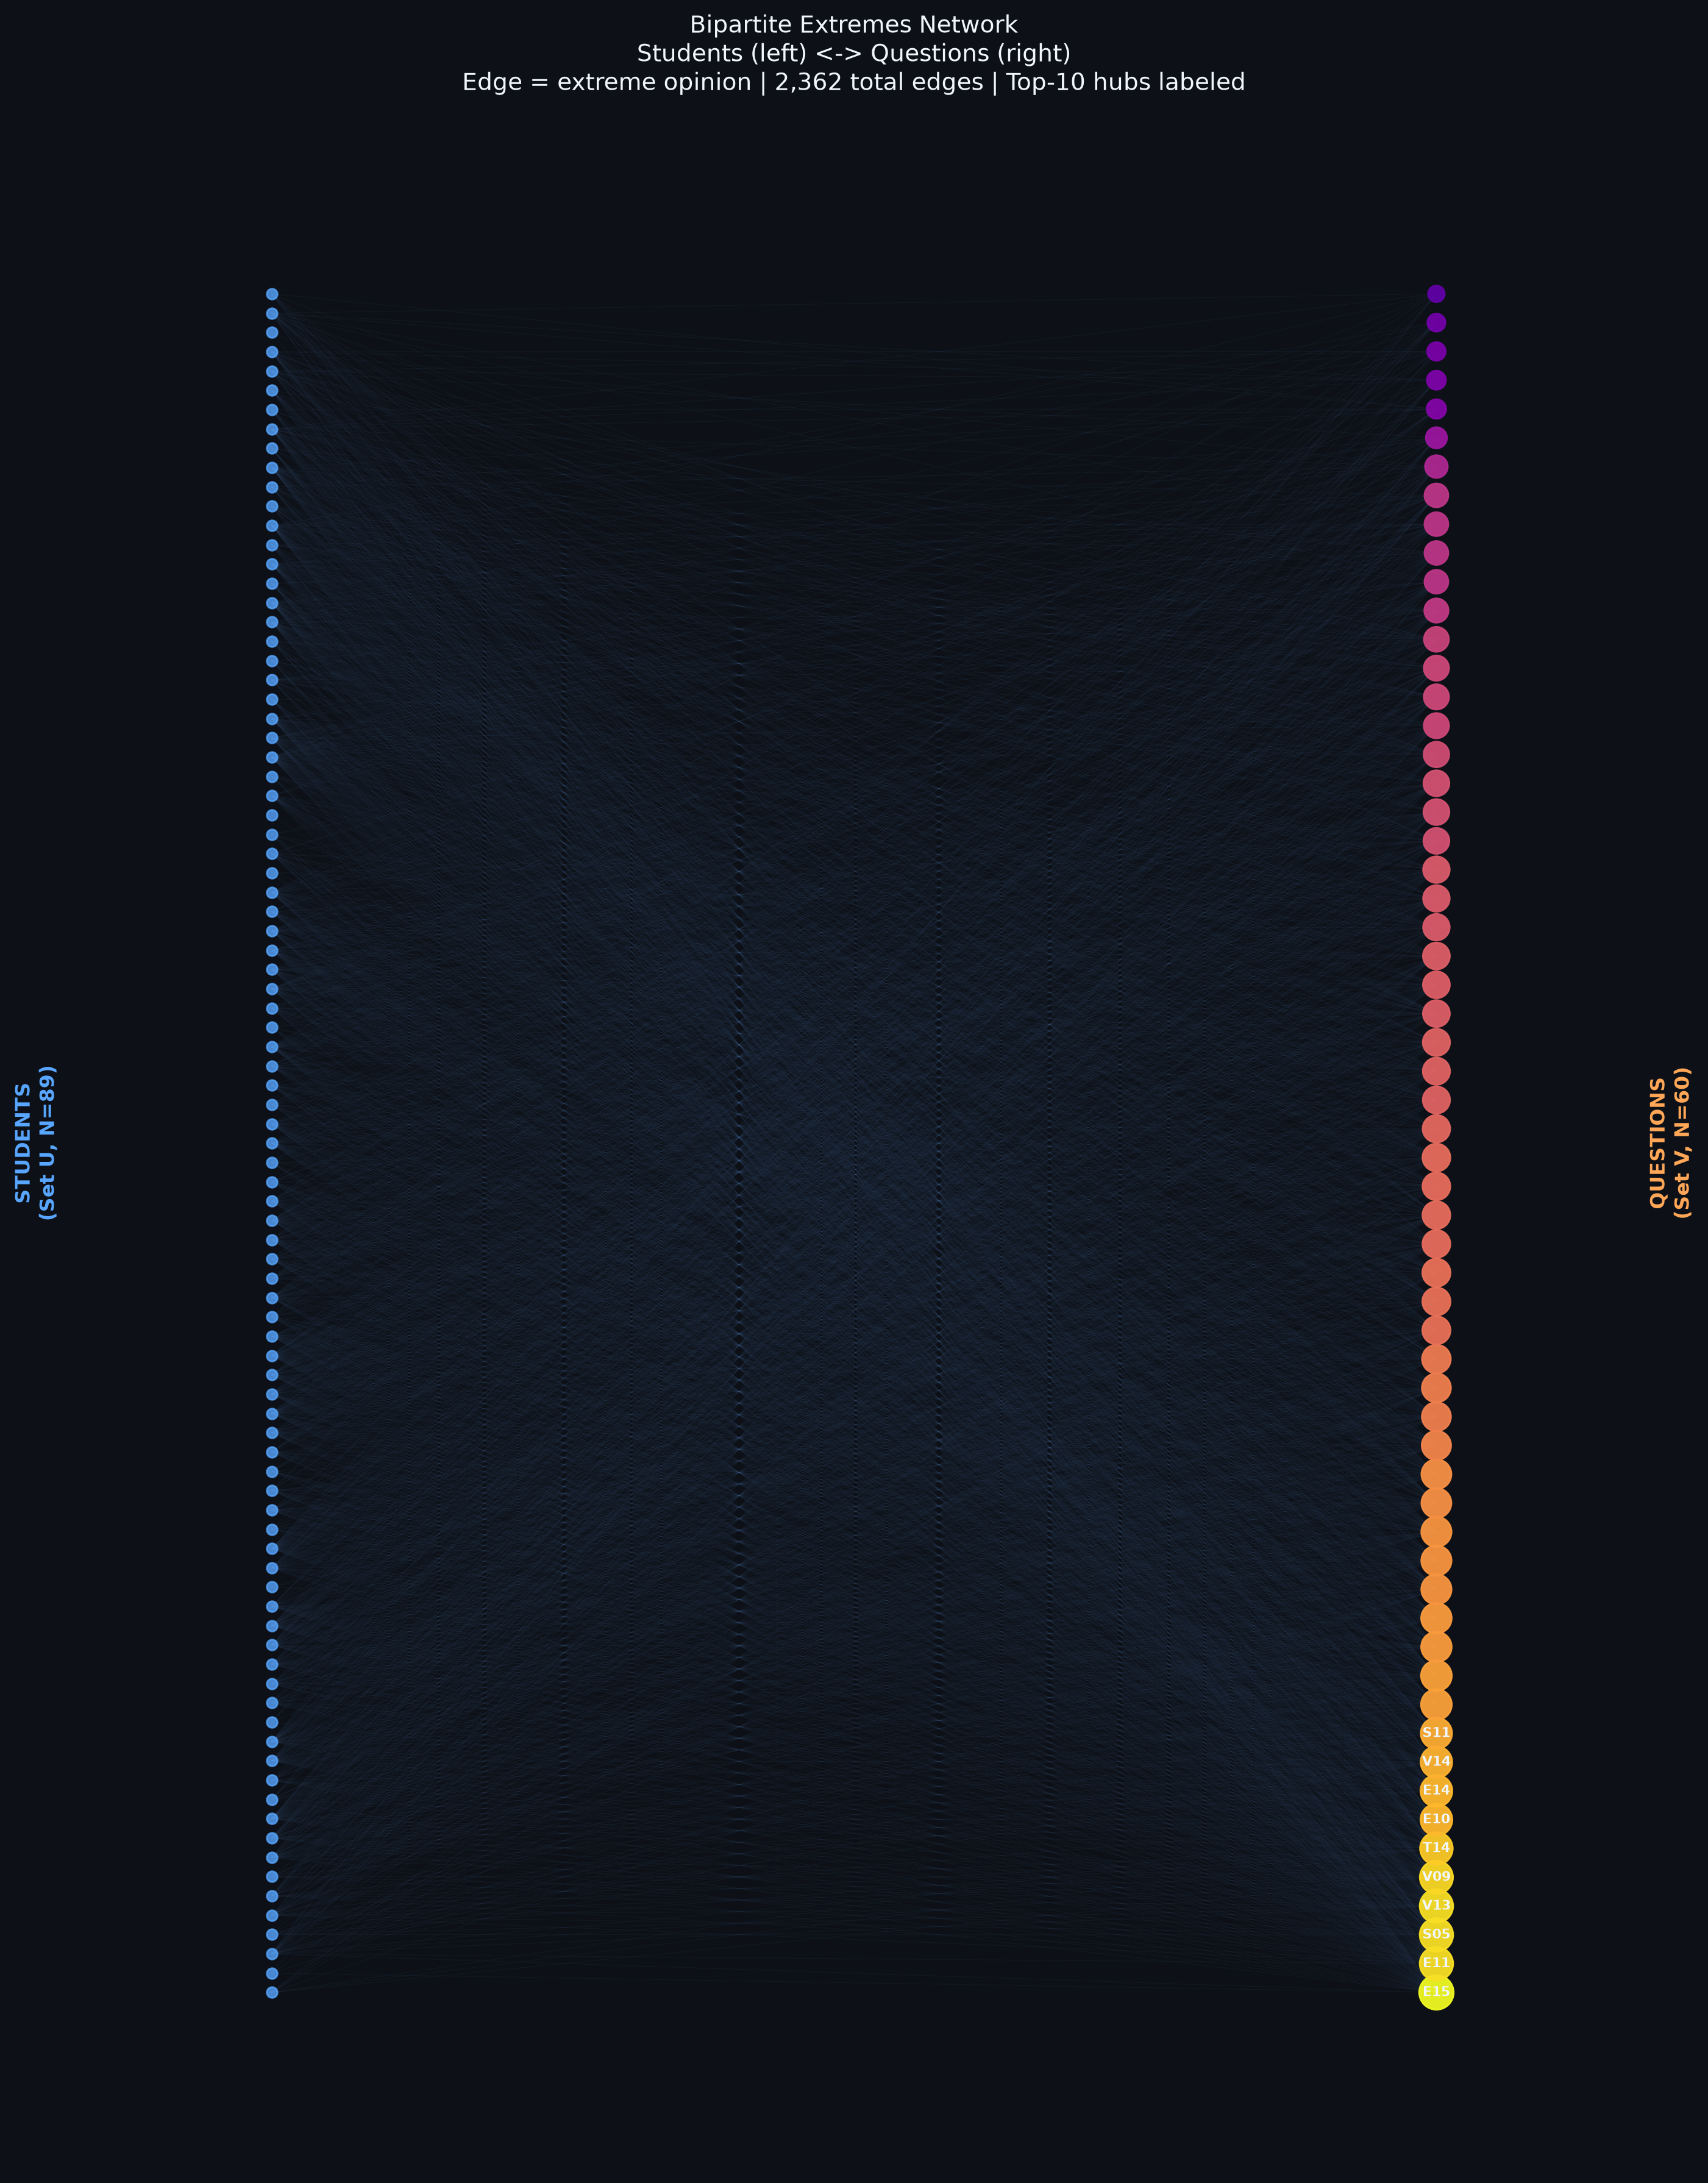
\includegraphics[width=0.48\textwidth]{Extreme Bipartite Network/extreme_plots/bipartite_layout.png} \hfill
    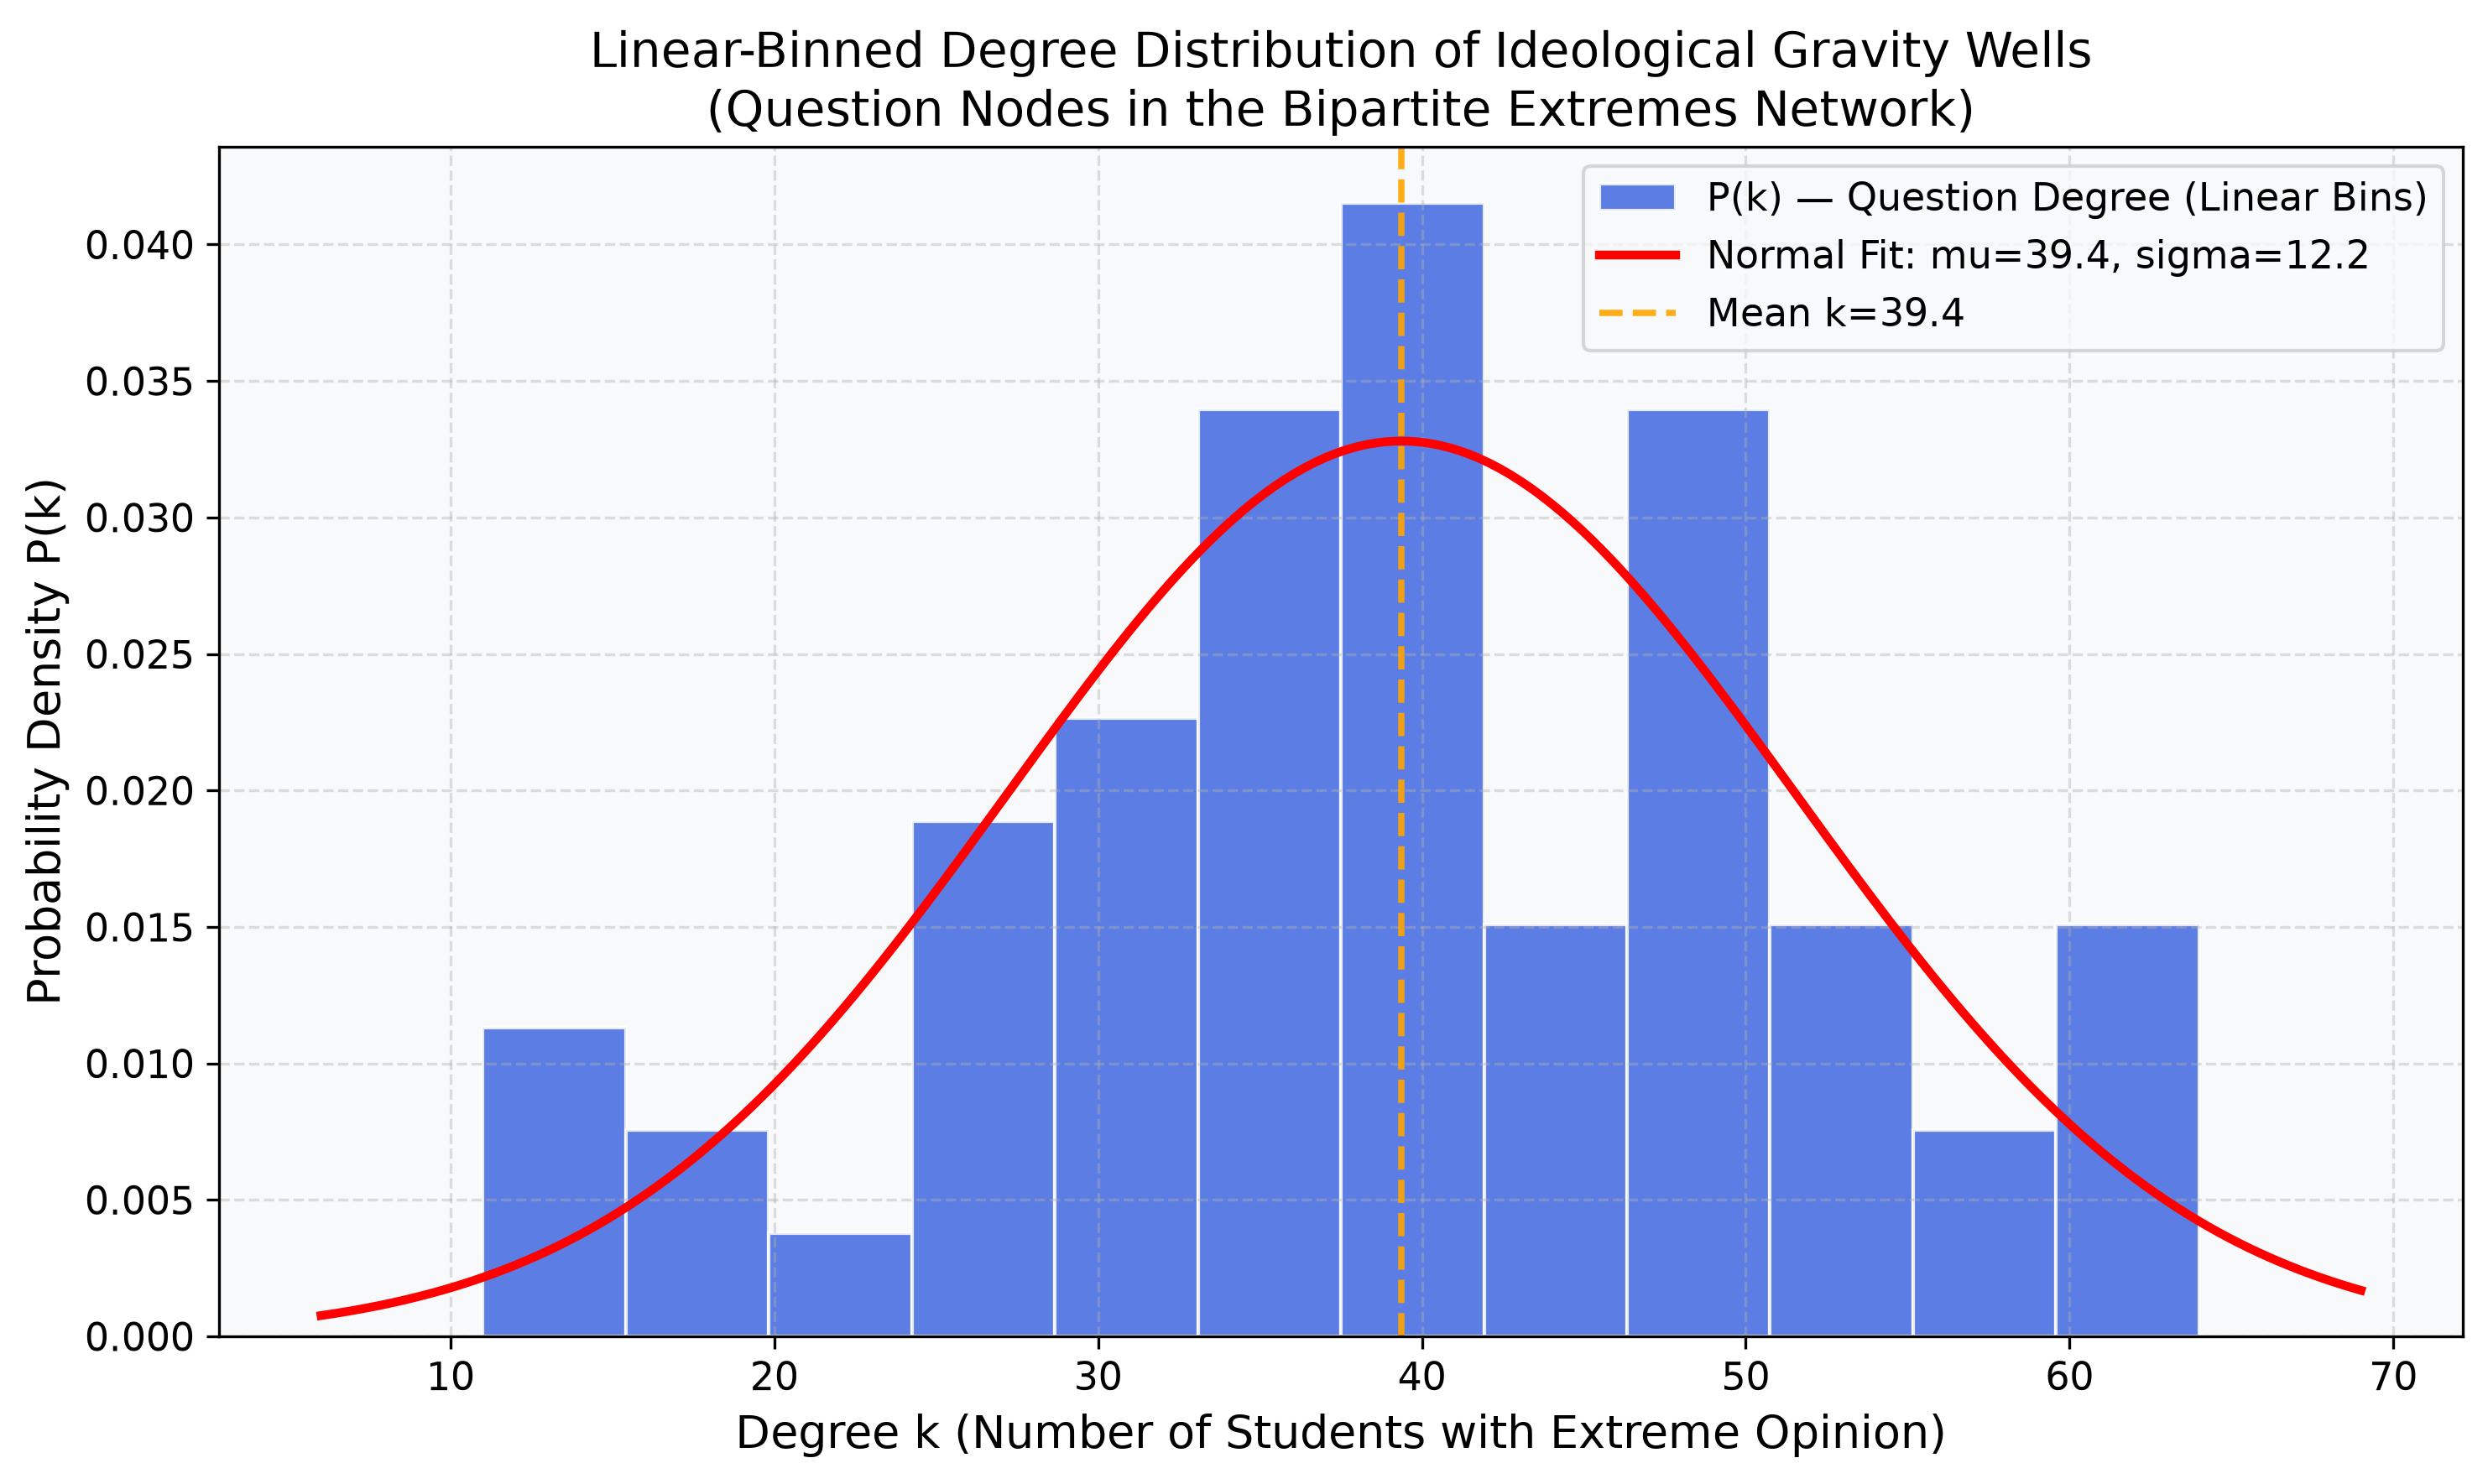
\includegraphics[width=0.48\textwidth]{Extreme Bipartite Network/extreme_plots/degree_distribution_linear.png}
    \caption{\textbf{Bipartite Network Layout and Degree Profile:} (Left) Bipartite graph connecting students (blue) to questions (plasma). (Right) Linear-binned degree distribution fitting a normal curve ($\mu = 39.37$, $\sigma = 12.16$).}
    \label{fig:bipartite_linear}
\end{figure}

\begin{figure}[H]
    \centering
    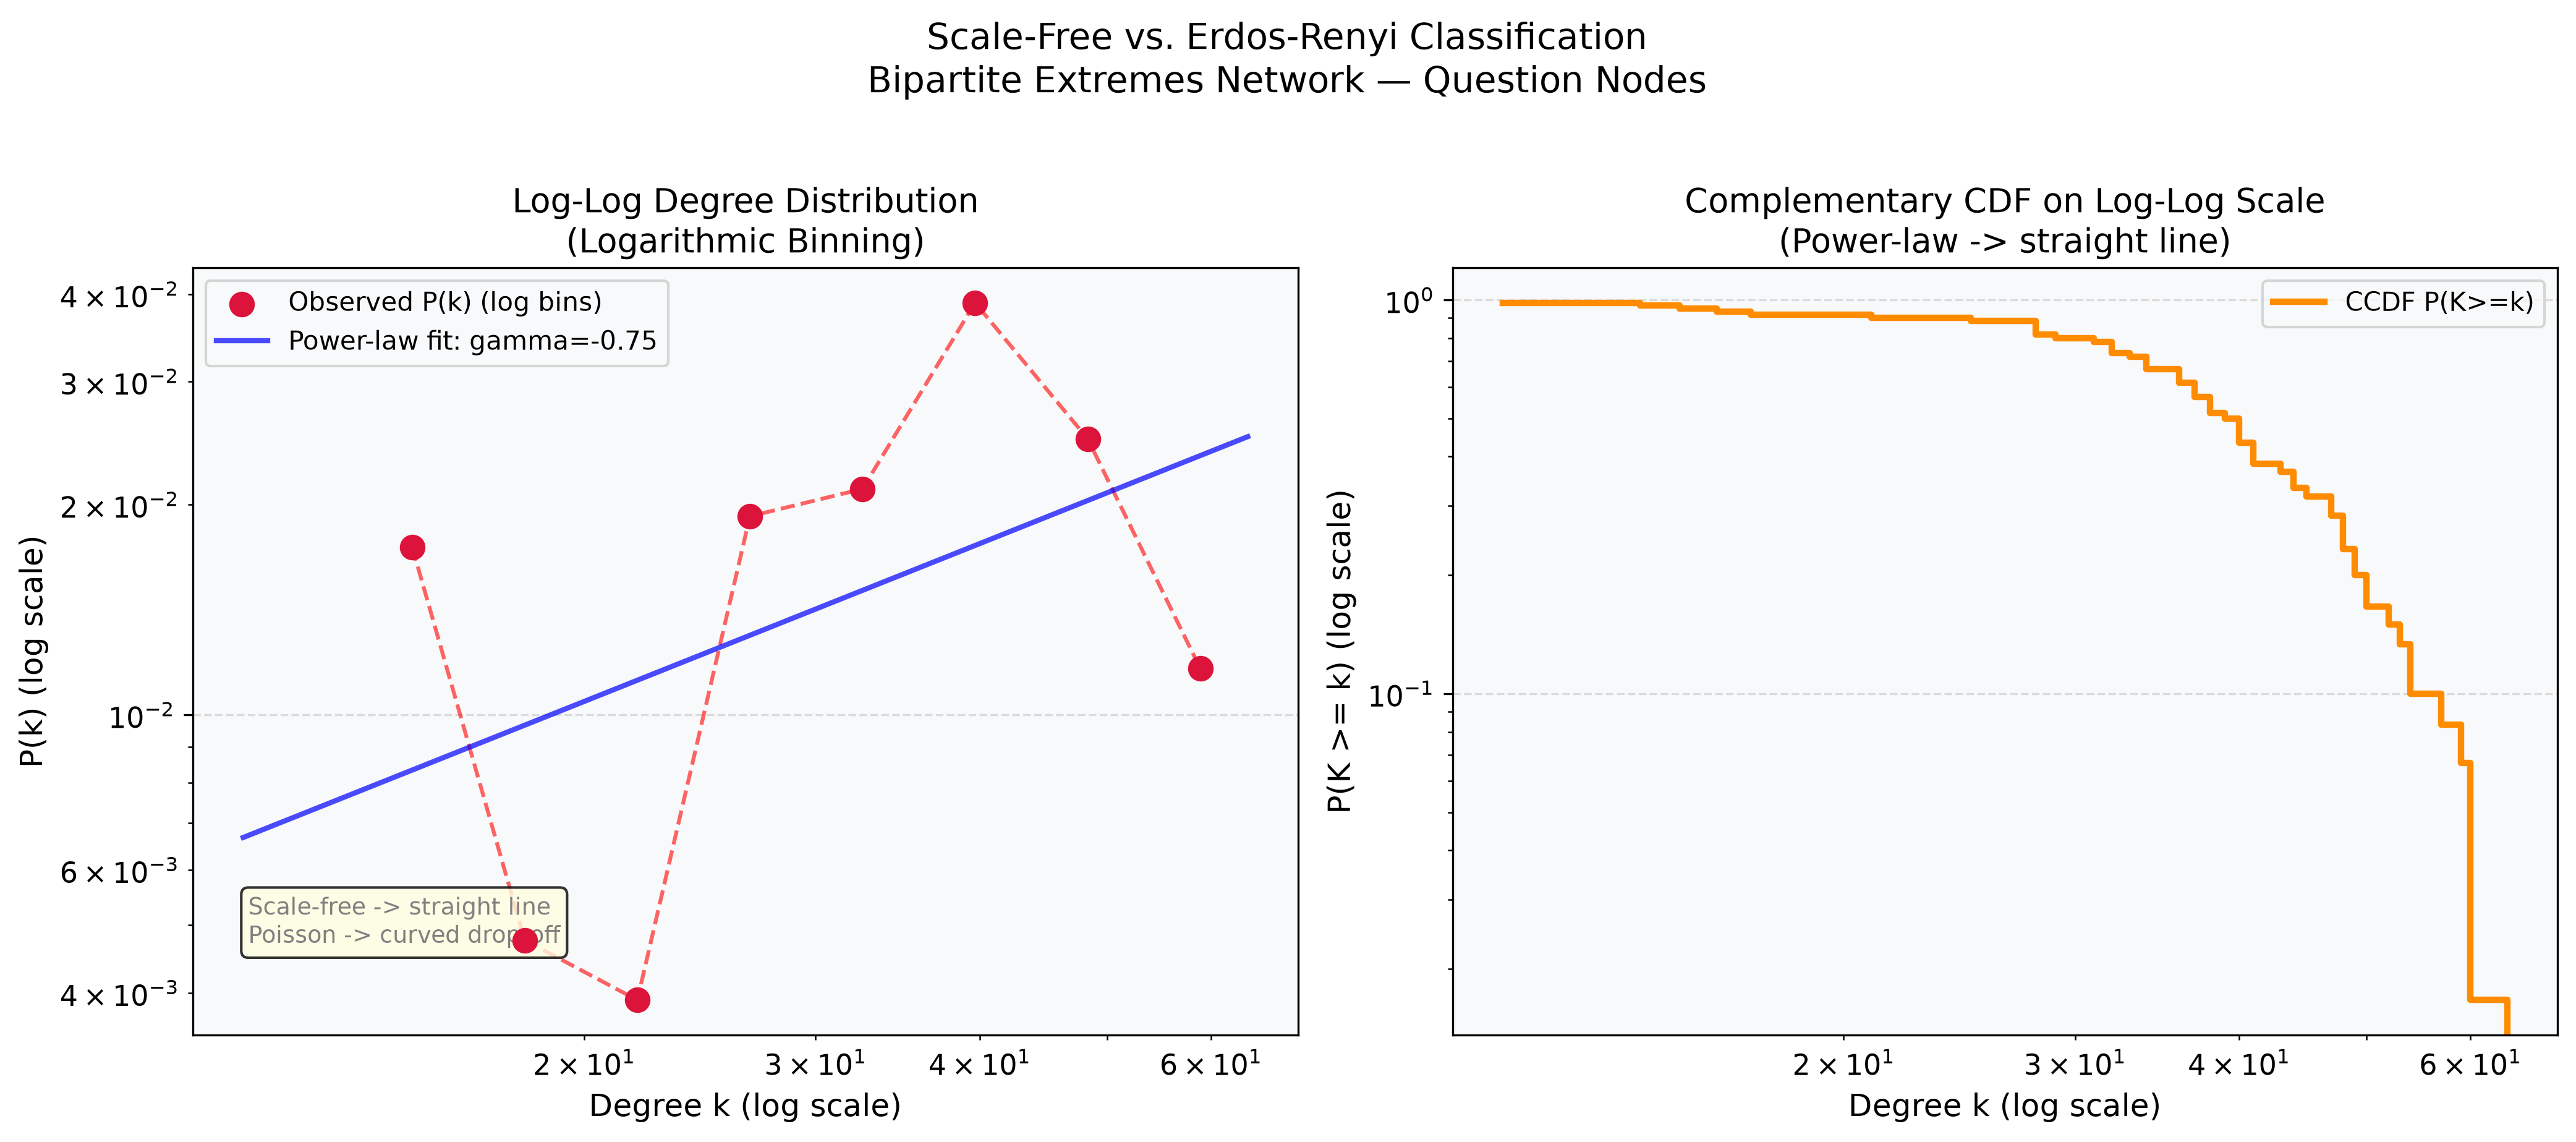
\includegraphics[width=0.48\textwidth]{Extreme Bipartite Network/extreme_plots/degree_distribution_loglog.png} \hfill
    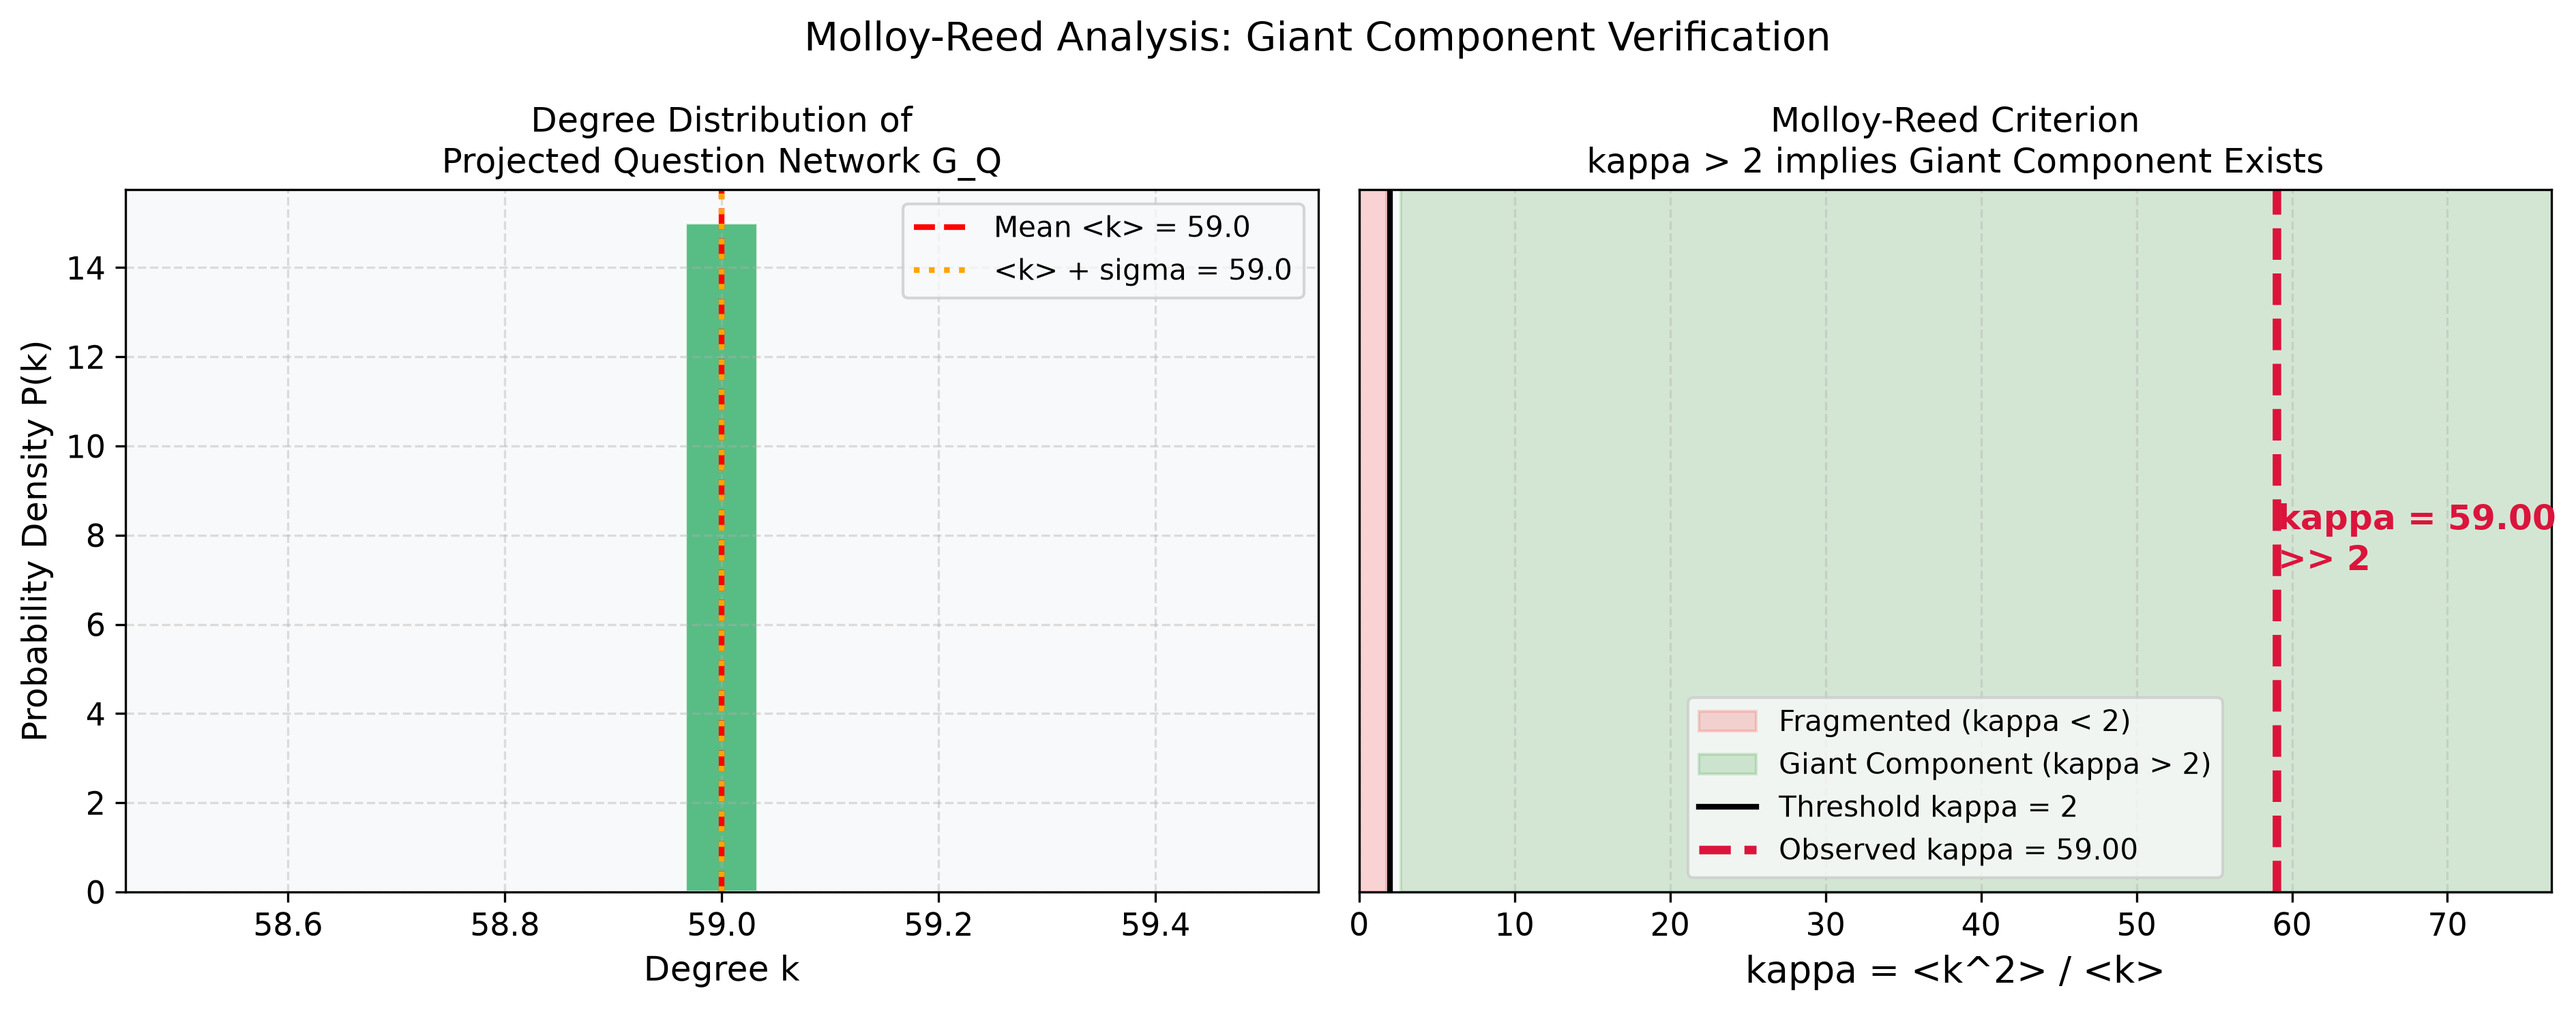
\includegraphics[width=0.48\textwidth]{Extreme Bipartite Network/extreme_plots/molloy_reed.png}
    \caption{\textbf{Topological Classification and Percolation Analysis:} (Left) Log-log degree distribution and CCDF confirming non-scale-free structure ($\hat{\gamma} = 0.750$). (Right) Molloy--Reed criterion ($\kappa = 59.0 \gg 2$) proving supercritical percolation.}
    \label{fig:bipartite_loglog_molloy}
\end{figure}

\begin{table}[H]
\centering
\small
\caption{Bipartite Extremes and Projected Graph Structural Parameters}
\label{tab:bipartite_params}
\begin{tabular}{llrl}
\toprule
\textbf{Parameter} & \textbf{Metric Name} & \textbf{Observed Value} & \textbf{Mathematical Implication} \\
\midrule
$N_U, N_V$ & Active Students / Questions & $89 \;/\; 60$ & Bipartite node partitions \\
$|E|$ & Extreme Opinions ($\tau \in \{1, 5\}$) & $2{,}362$ edges & Density $\delta = 0.4423$ \\
$\hat{\gamma}$ & Power-Law Degree Exponent & $0.750$ & Rules out scale-free topology ($2 < \gamma < 3$) \\
$\sigma^2_k / \langle k \rangle$ & Degree Dispersion Index & $3.75$ & Overdispersed bounded distribution \\
$\kappa$ & Molloy--Reed Parameter & $\mathbf{59.000} \gg 2$ & Supercritical percolation guaranteed \\
$G_Q$ & Projected Question Graph & Complete $K_{60}$ & Universal cross-domain co-occurrence \\
\bottomrule
\end{tabular}
\end{table}

\textbf{Topological Findings:}
\begin{itemize}
    \setlength{\itemsep}{0pt}
    \item \textbf{Absence of Mega-Hubs:} The degree distribution has mean $\mu = 39.37$ and variance $\sigma^2 = 147.87$. The dispersion index ($\sigma^2 / \mu = 3.75$) indicates an overdispersed, bounded distribution rather than an Erd\H{o}s--R\'enyi random graph. The best-fit power law $\hat{\gamma} = 0.750 \notin [2, 3]$ and steep CCDF cliff drop definitively rule out a scale-free topology.
    \item \textbf{Complete Projection ($G_Q = K_{60}$):} Every question pair shares at least one student with an extreme view on both ($\delta = 1.0000$), proving absolute cross-cutting ideological cohesion.
    \item \textbf{Molloy--Reed Percolation:} $\kappa = 59.000 \gg 2$, confirming maximal percolation. Targeted attacks on polarizing questions are mathematically indistinguishable from random node failure, conferring absolute topological resilience.
    \item \textbf{Keystone Trio:} Strength centrality on $G_Q^W$ identifies \textbf{E15} (1.000, 71.9\% extreme), \textbf{E11} (0.988), and \textbf{V13} (0.979) as the primary anchors of cohort passion.
\end{itemize}

\begin{figure}[H]
    \centering
    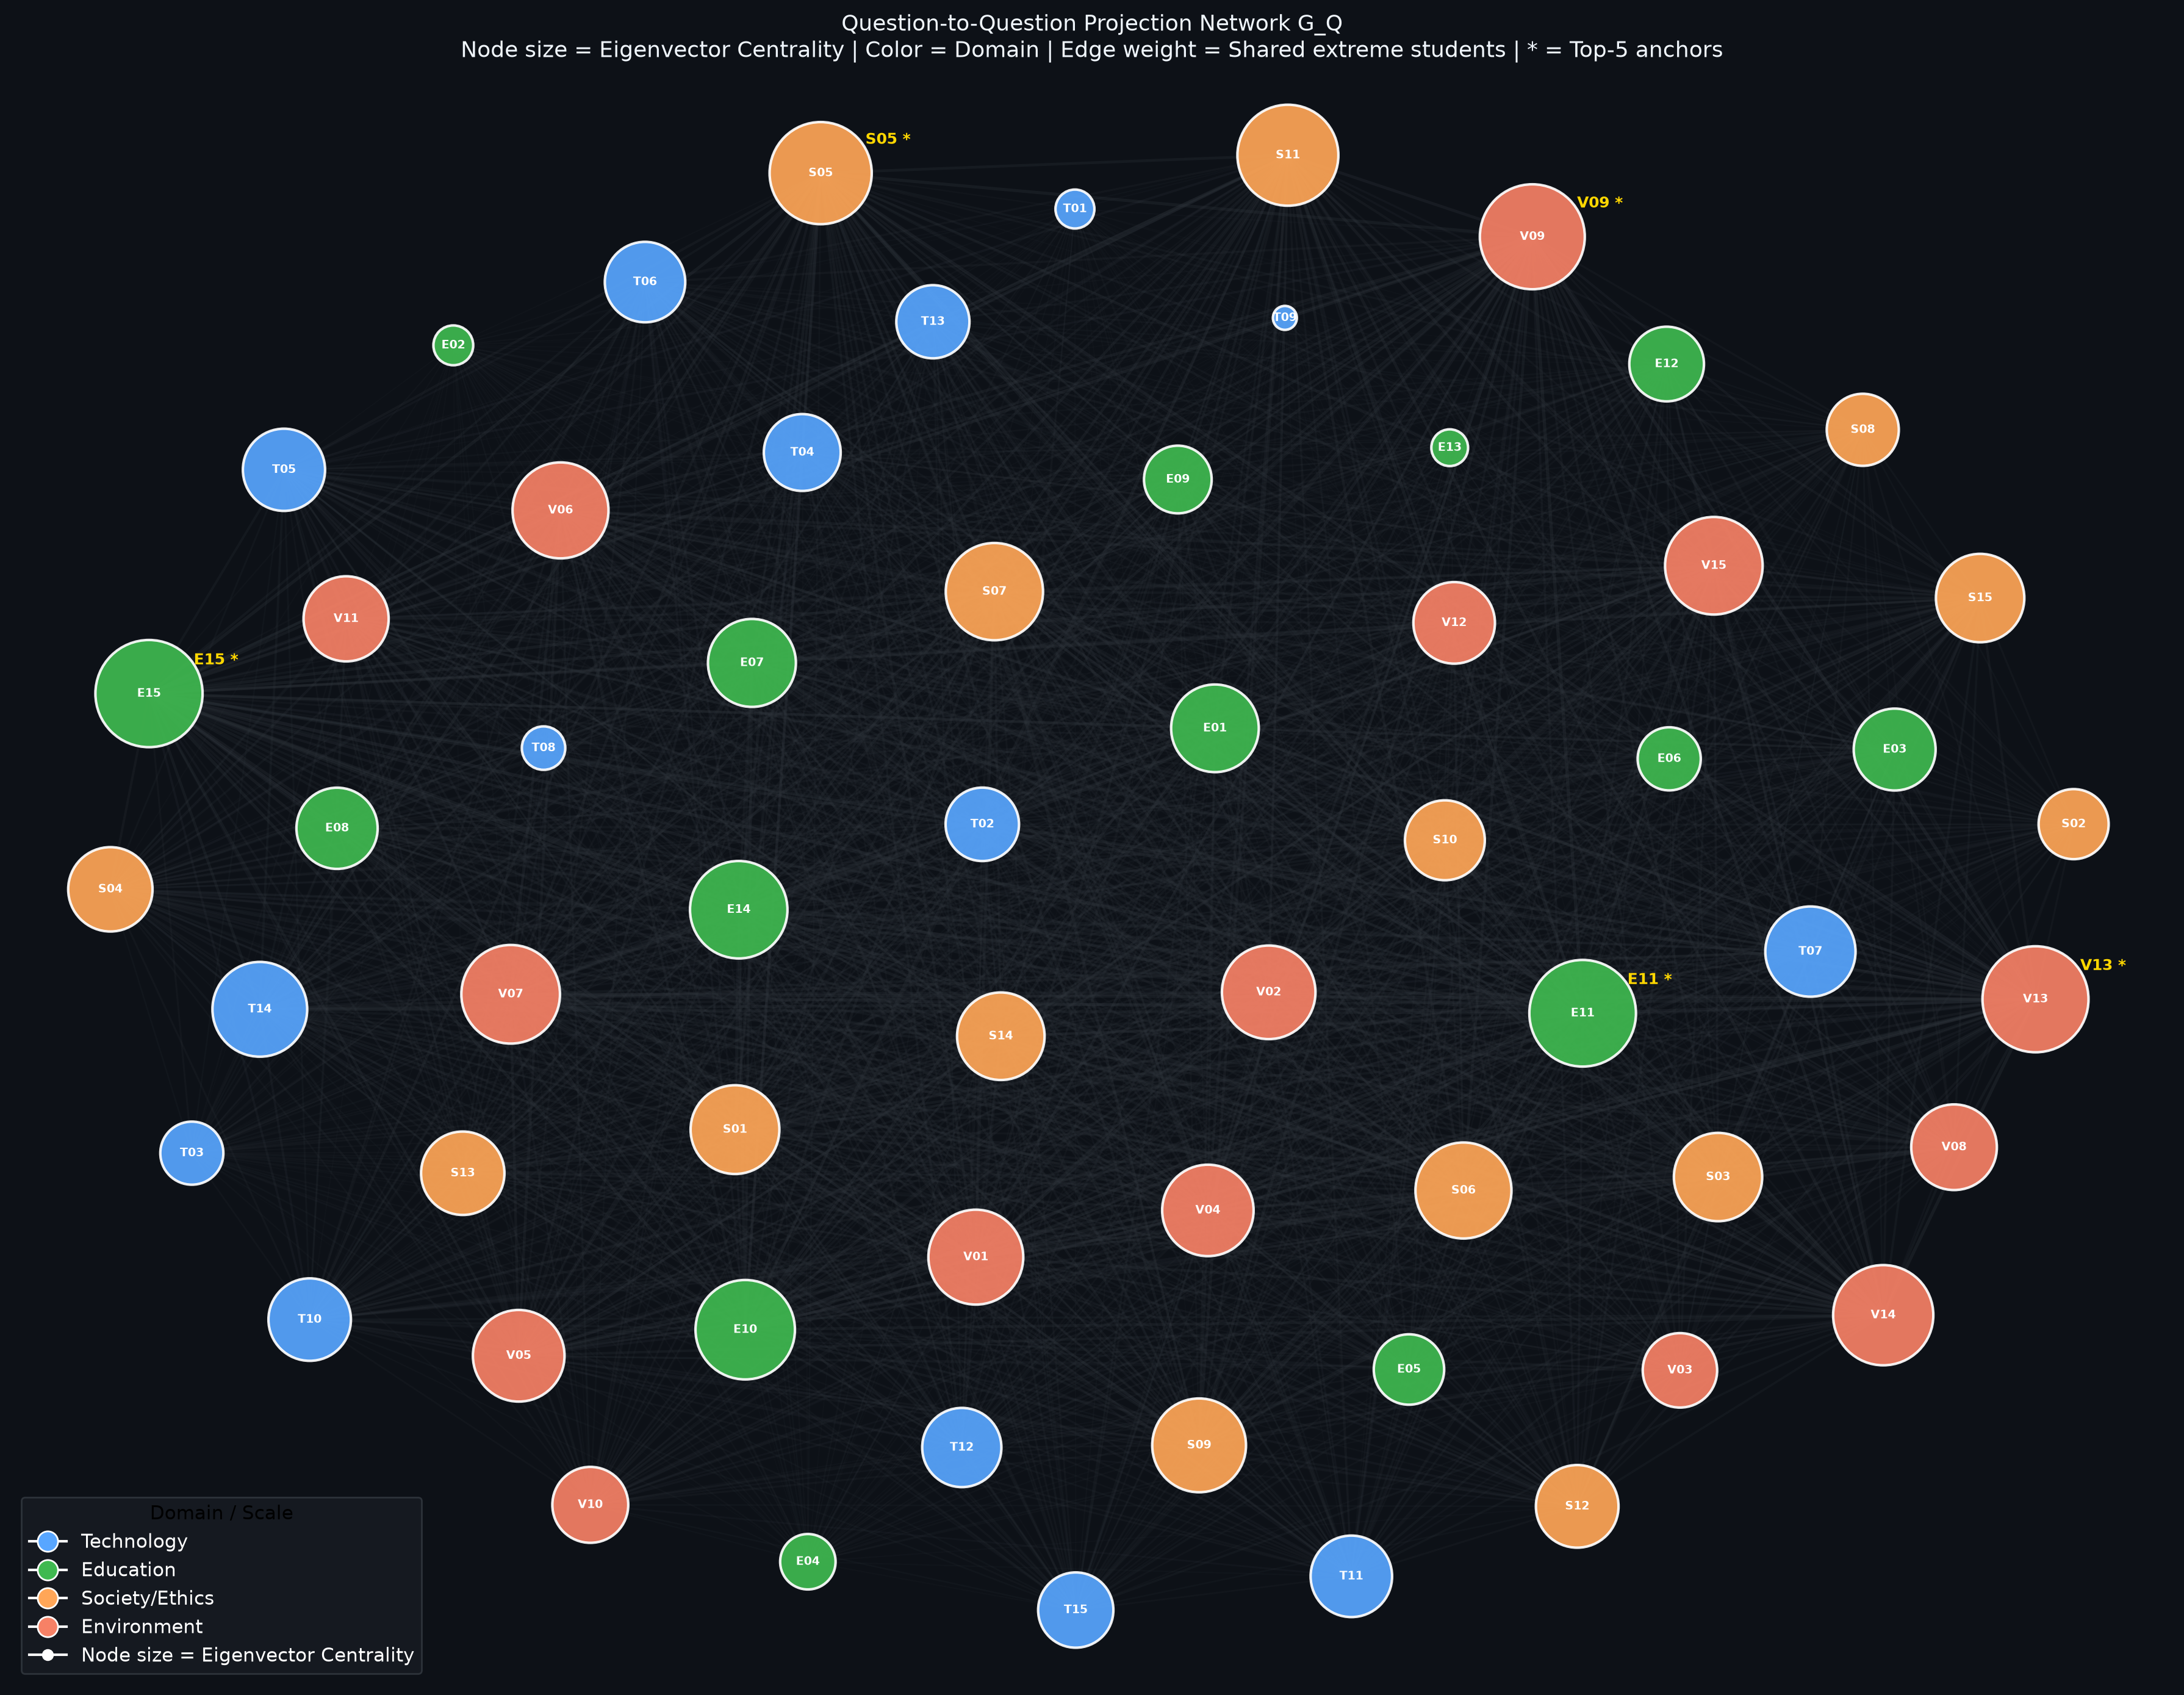
\includegraphics[width=0.48\textwidth]{Extreme Bipartite Network/extreme_plots/projected_network.png} \hfill
    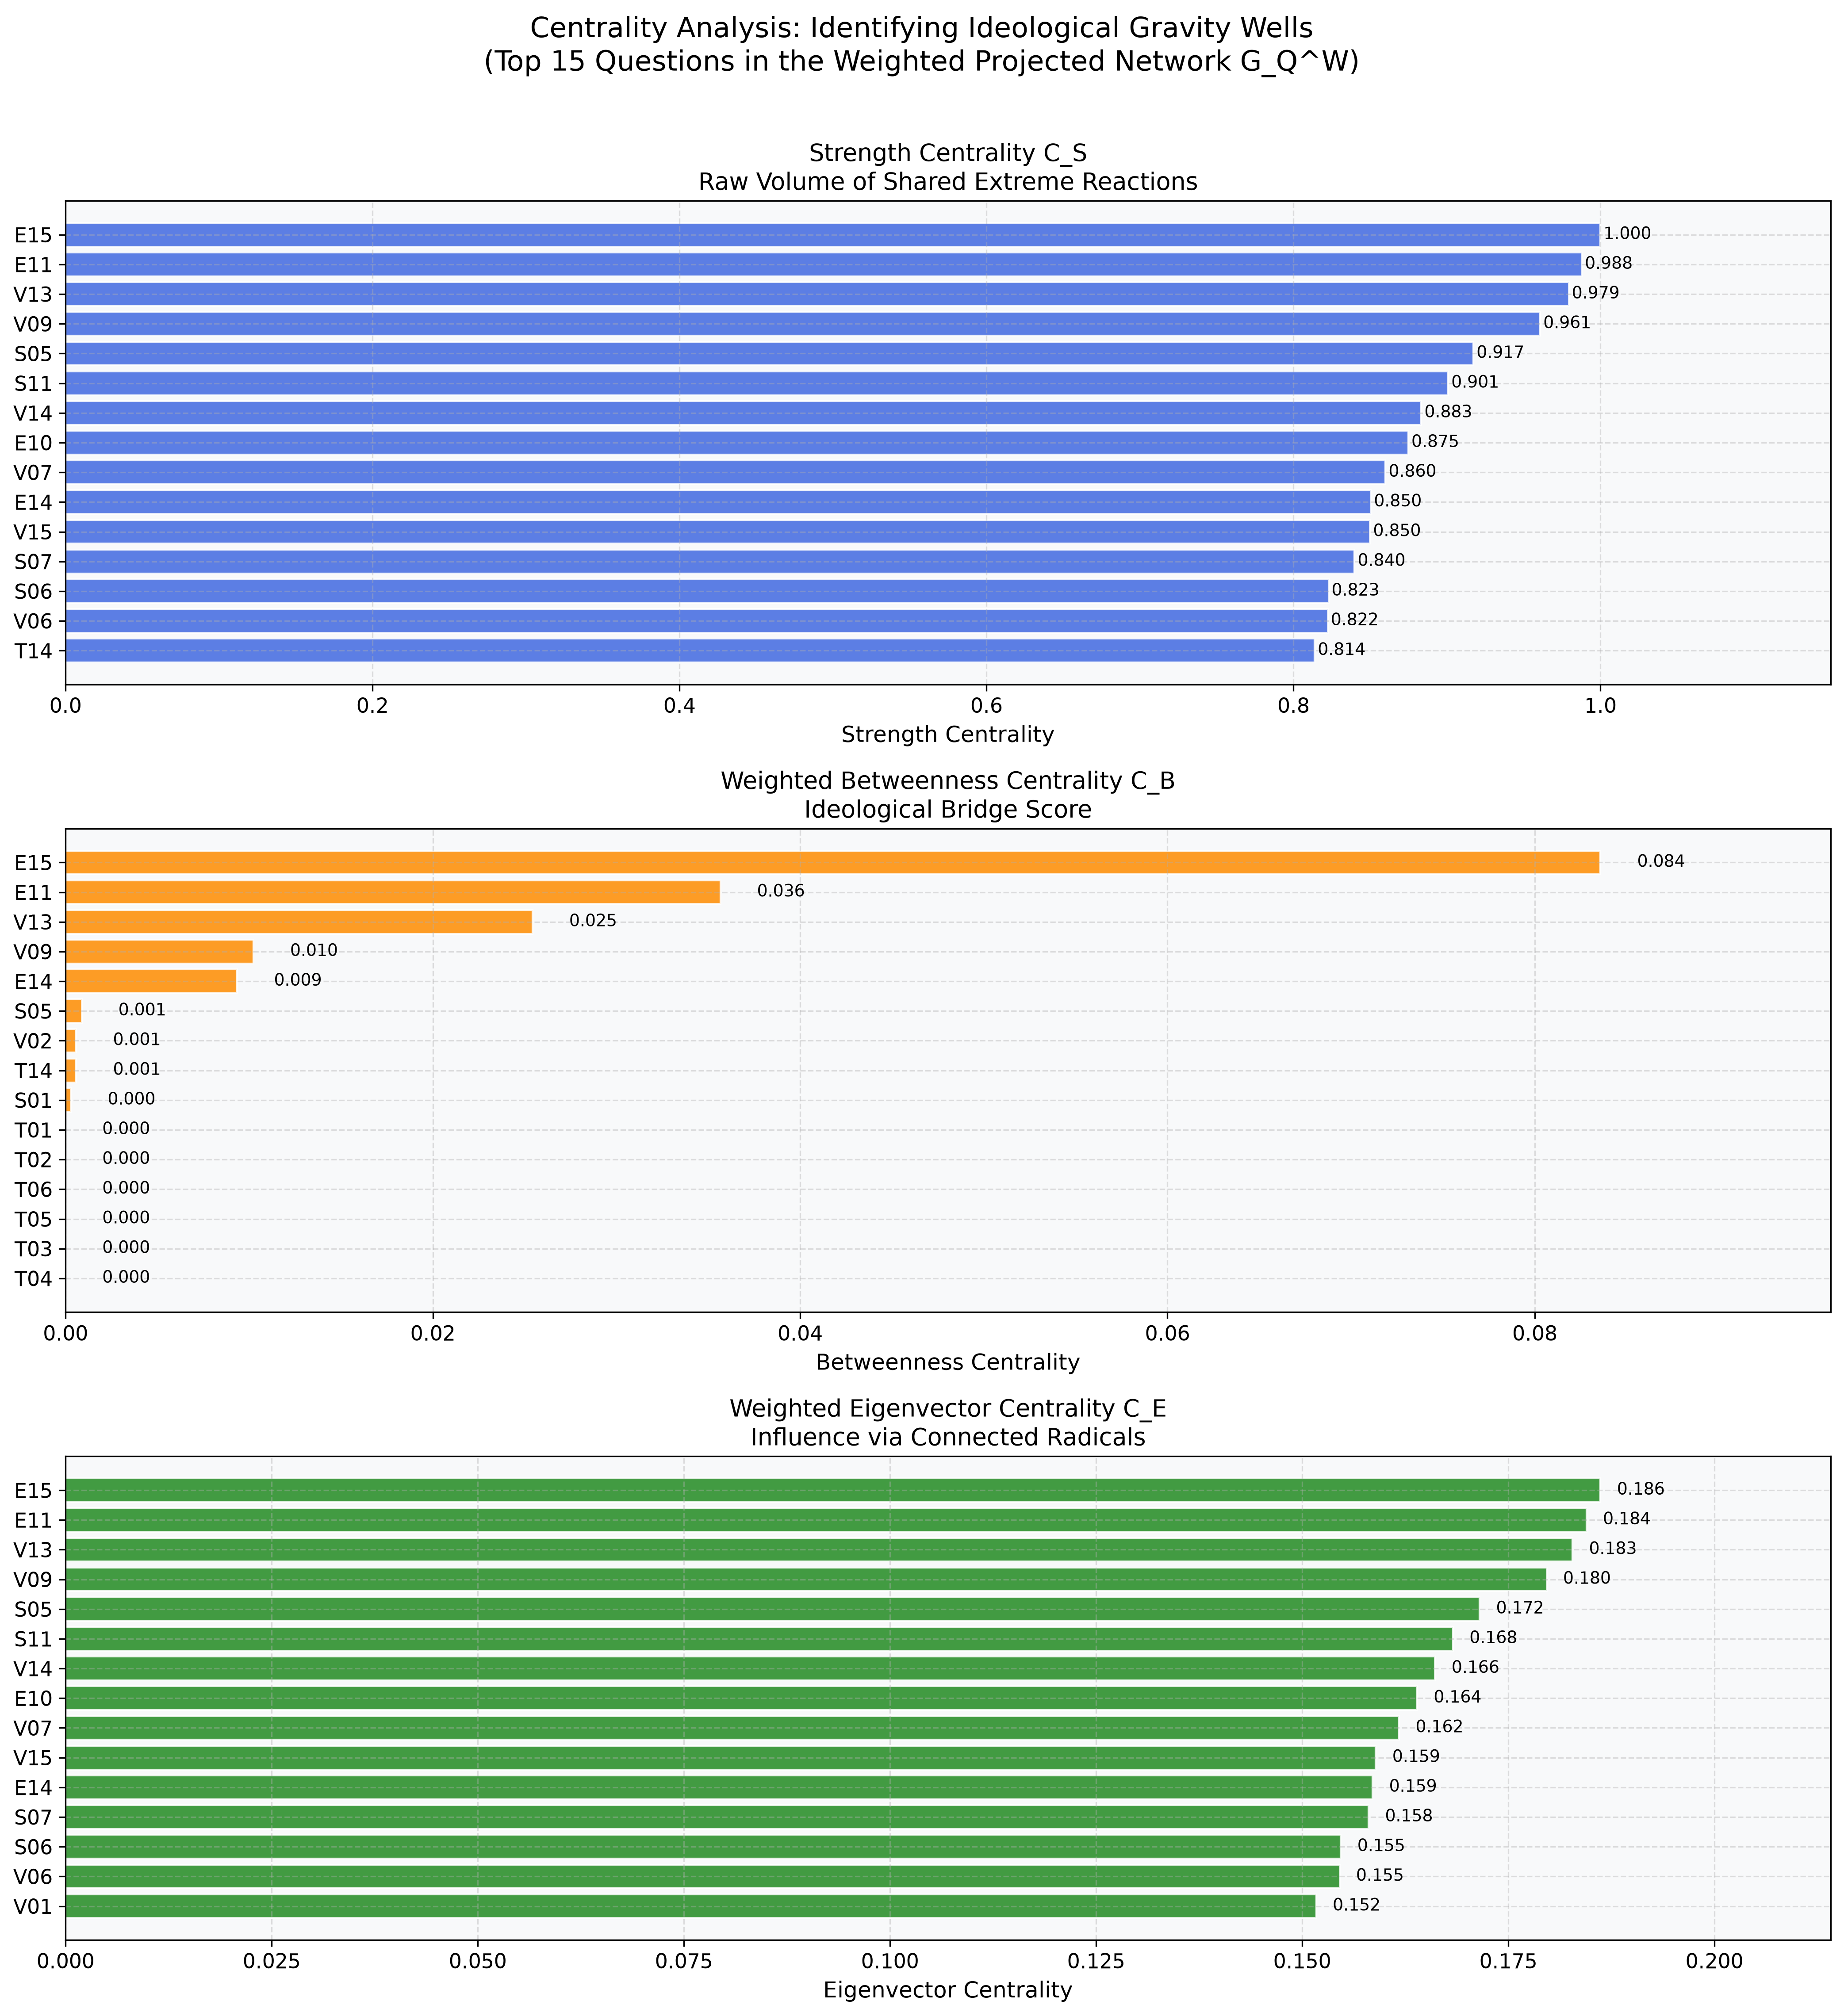
\includegraphics[width=0.48\textwidth]{Extreme Bipartite Network/extreme_plots/centrality_bars.png}
    \caption{\textbf{Question Projection and Centrality Spectrum:} (Left) Complete projection graph $G_Q = K_{60}$. (Right) Weighted centrality distributions highlighting the Keystone Trio (\texttt{E15}, \texttt{E11}, \texttt{V13}).}
    \label{fig:bipartite_proj_bars}
\end{figure}

\subsection{Question--Question Correlation Network: Anchors, Bridges, and Modularity}
Filtering Spearman rank correlations at $\rho > 0.35$ eliminates ambient consensus noise, isolating 188 suprathreshold edges across 60 questions ($\mathcal{D} = 0.1062$), a 47-node giant component, and 13 isolated questions representing polarizing or niche issues (\texttt{T04}, \texttt{T08}, \texttt{E02}, \texttt{E08}, \texttt{S08}, etc.).

\begin{figure}[H]
    \centering
    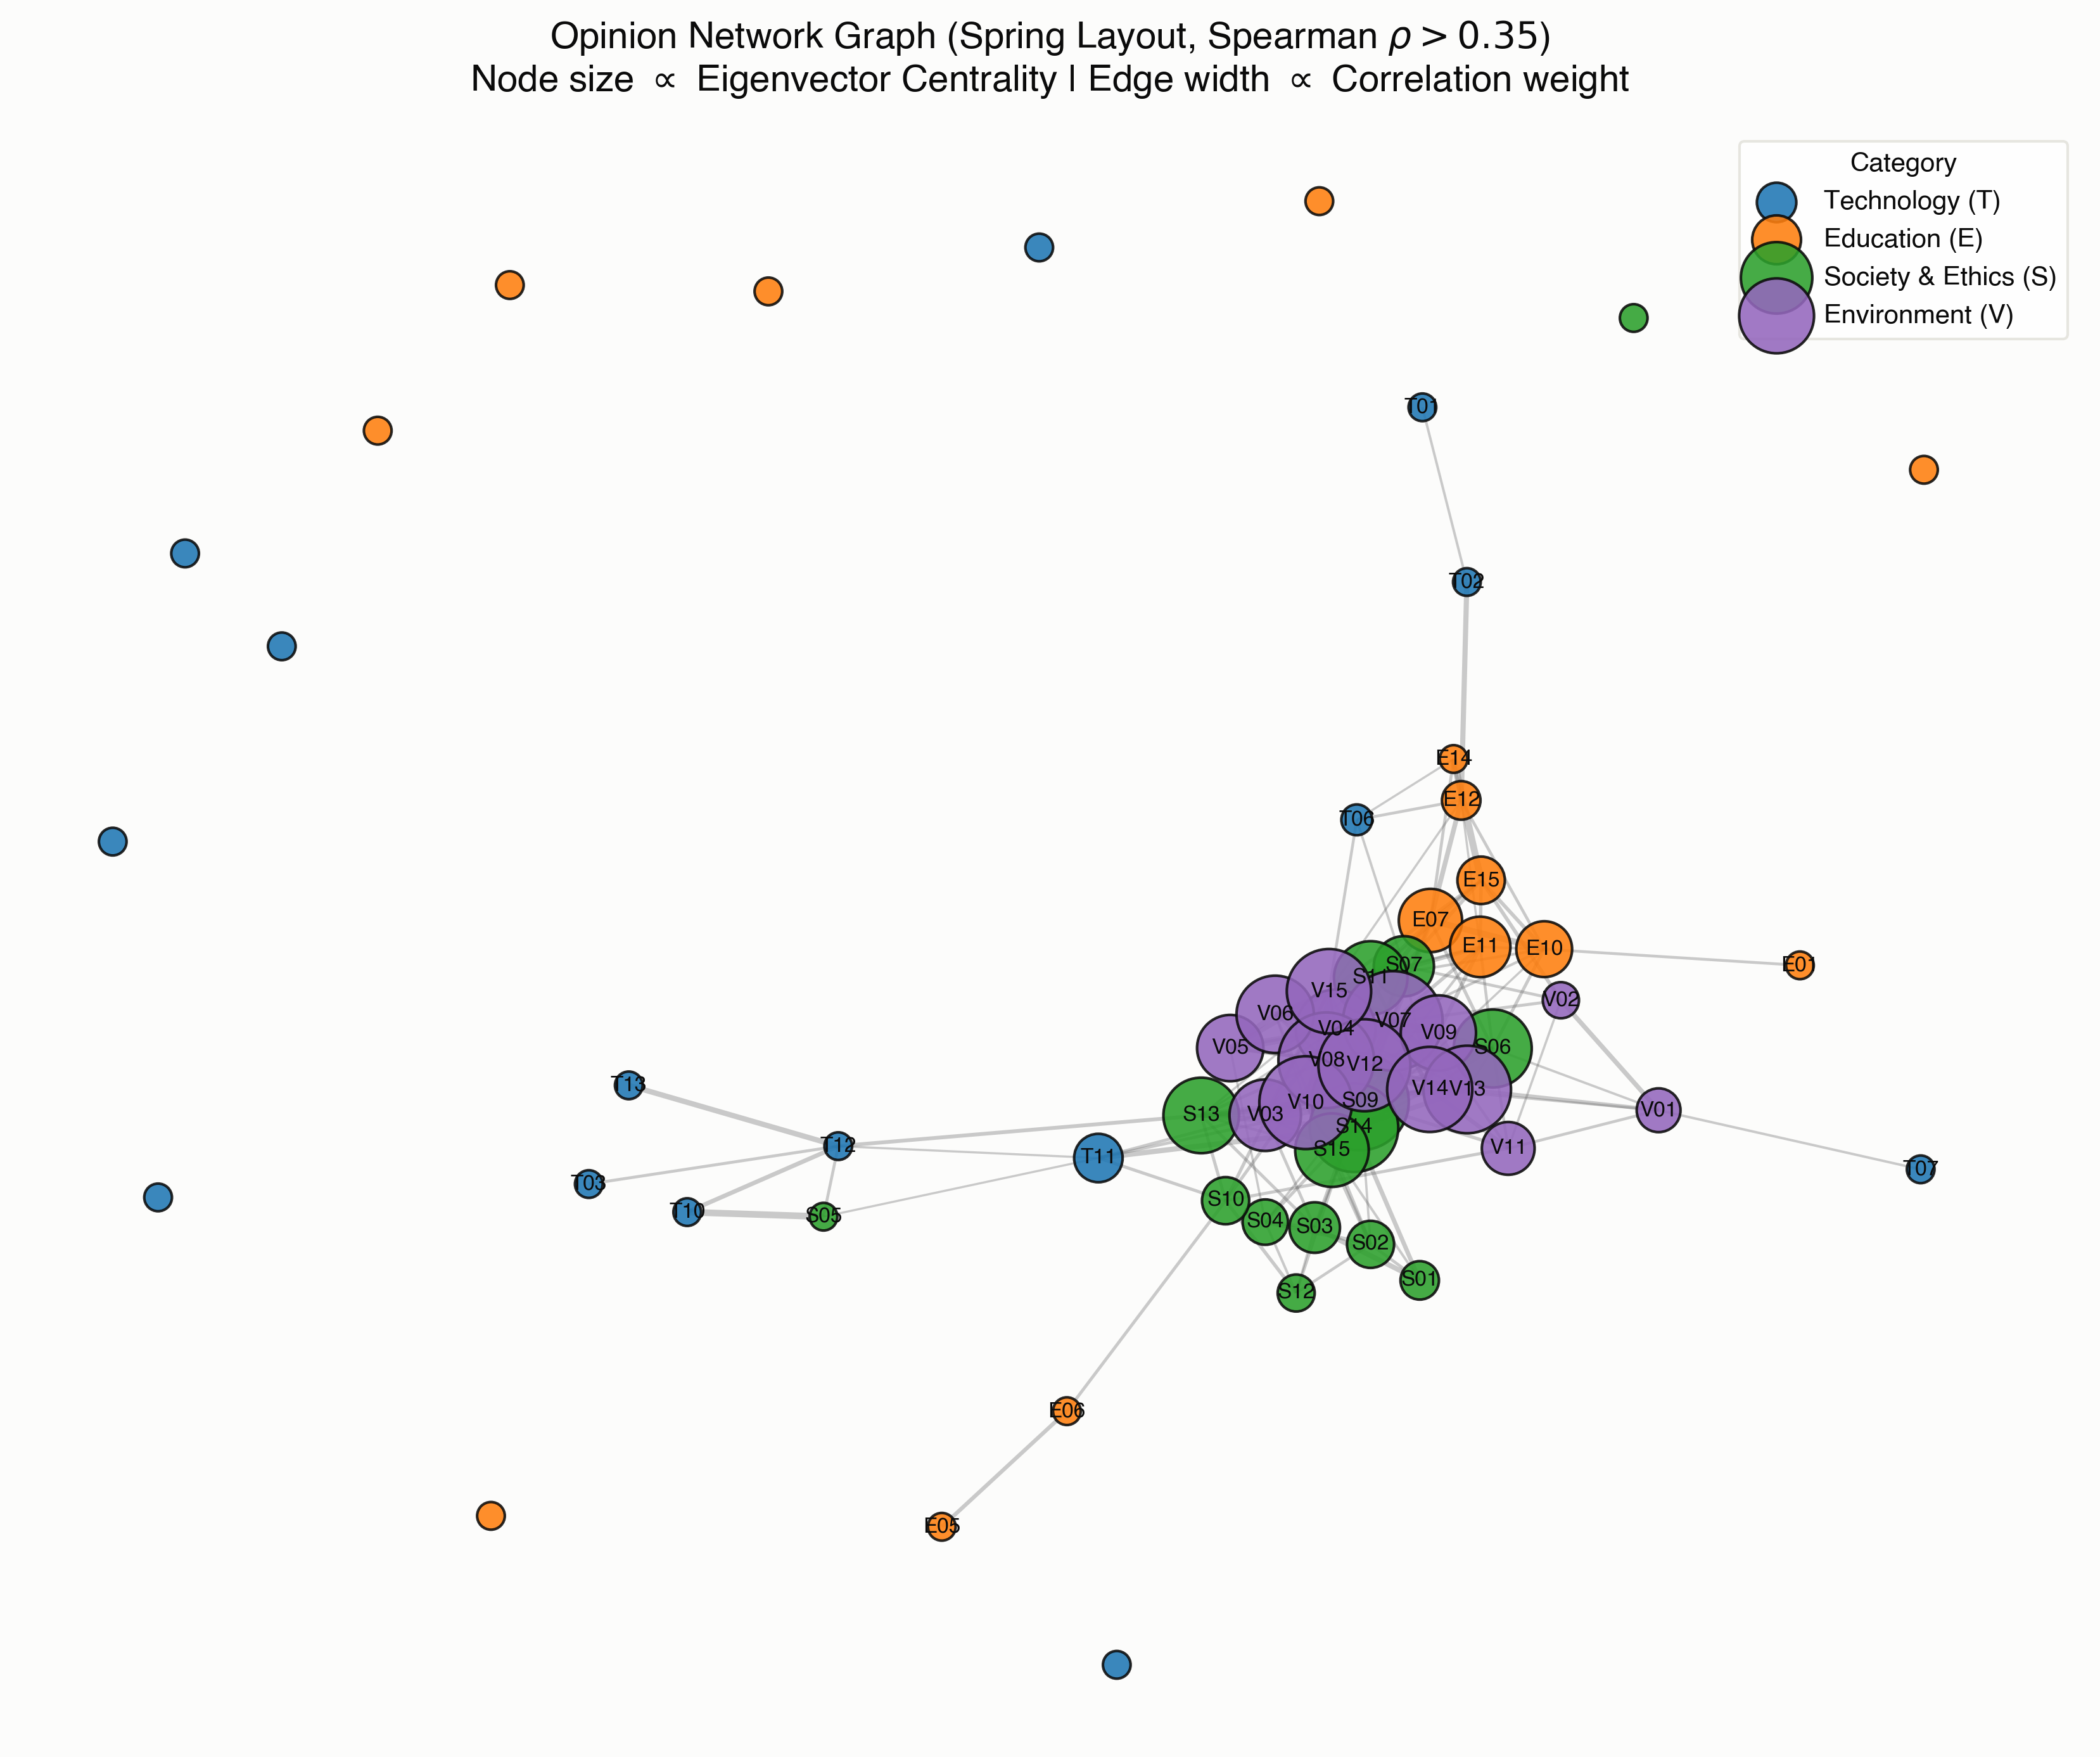
\includegraphics[width=0.48\textwidth]{Question Network/network_graph.png} \hfill
    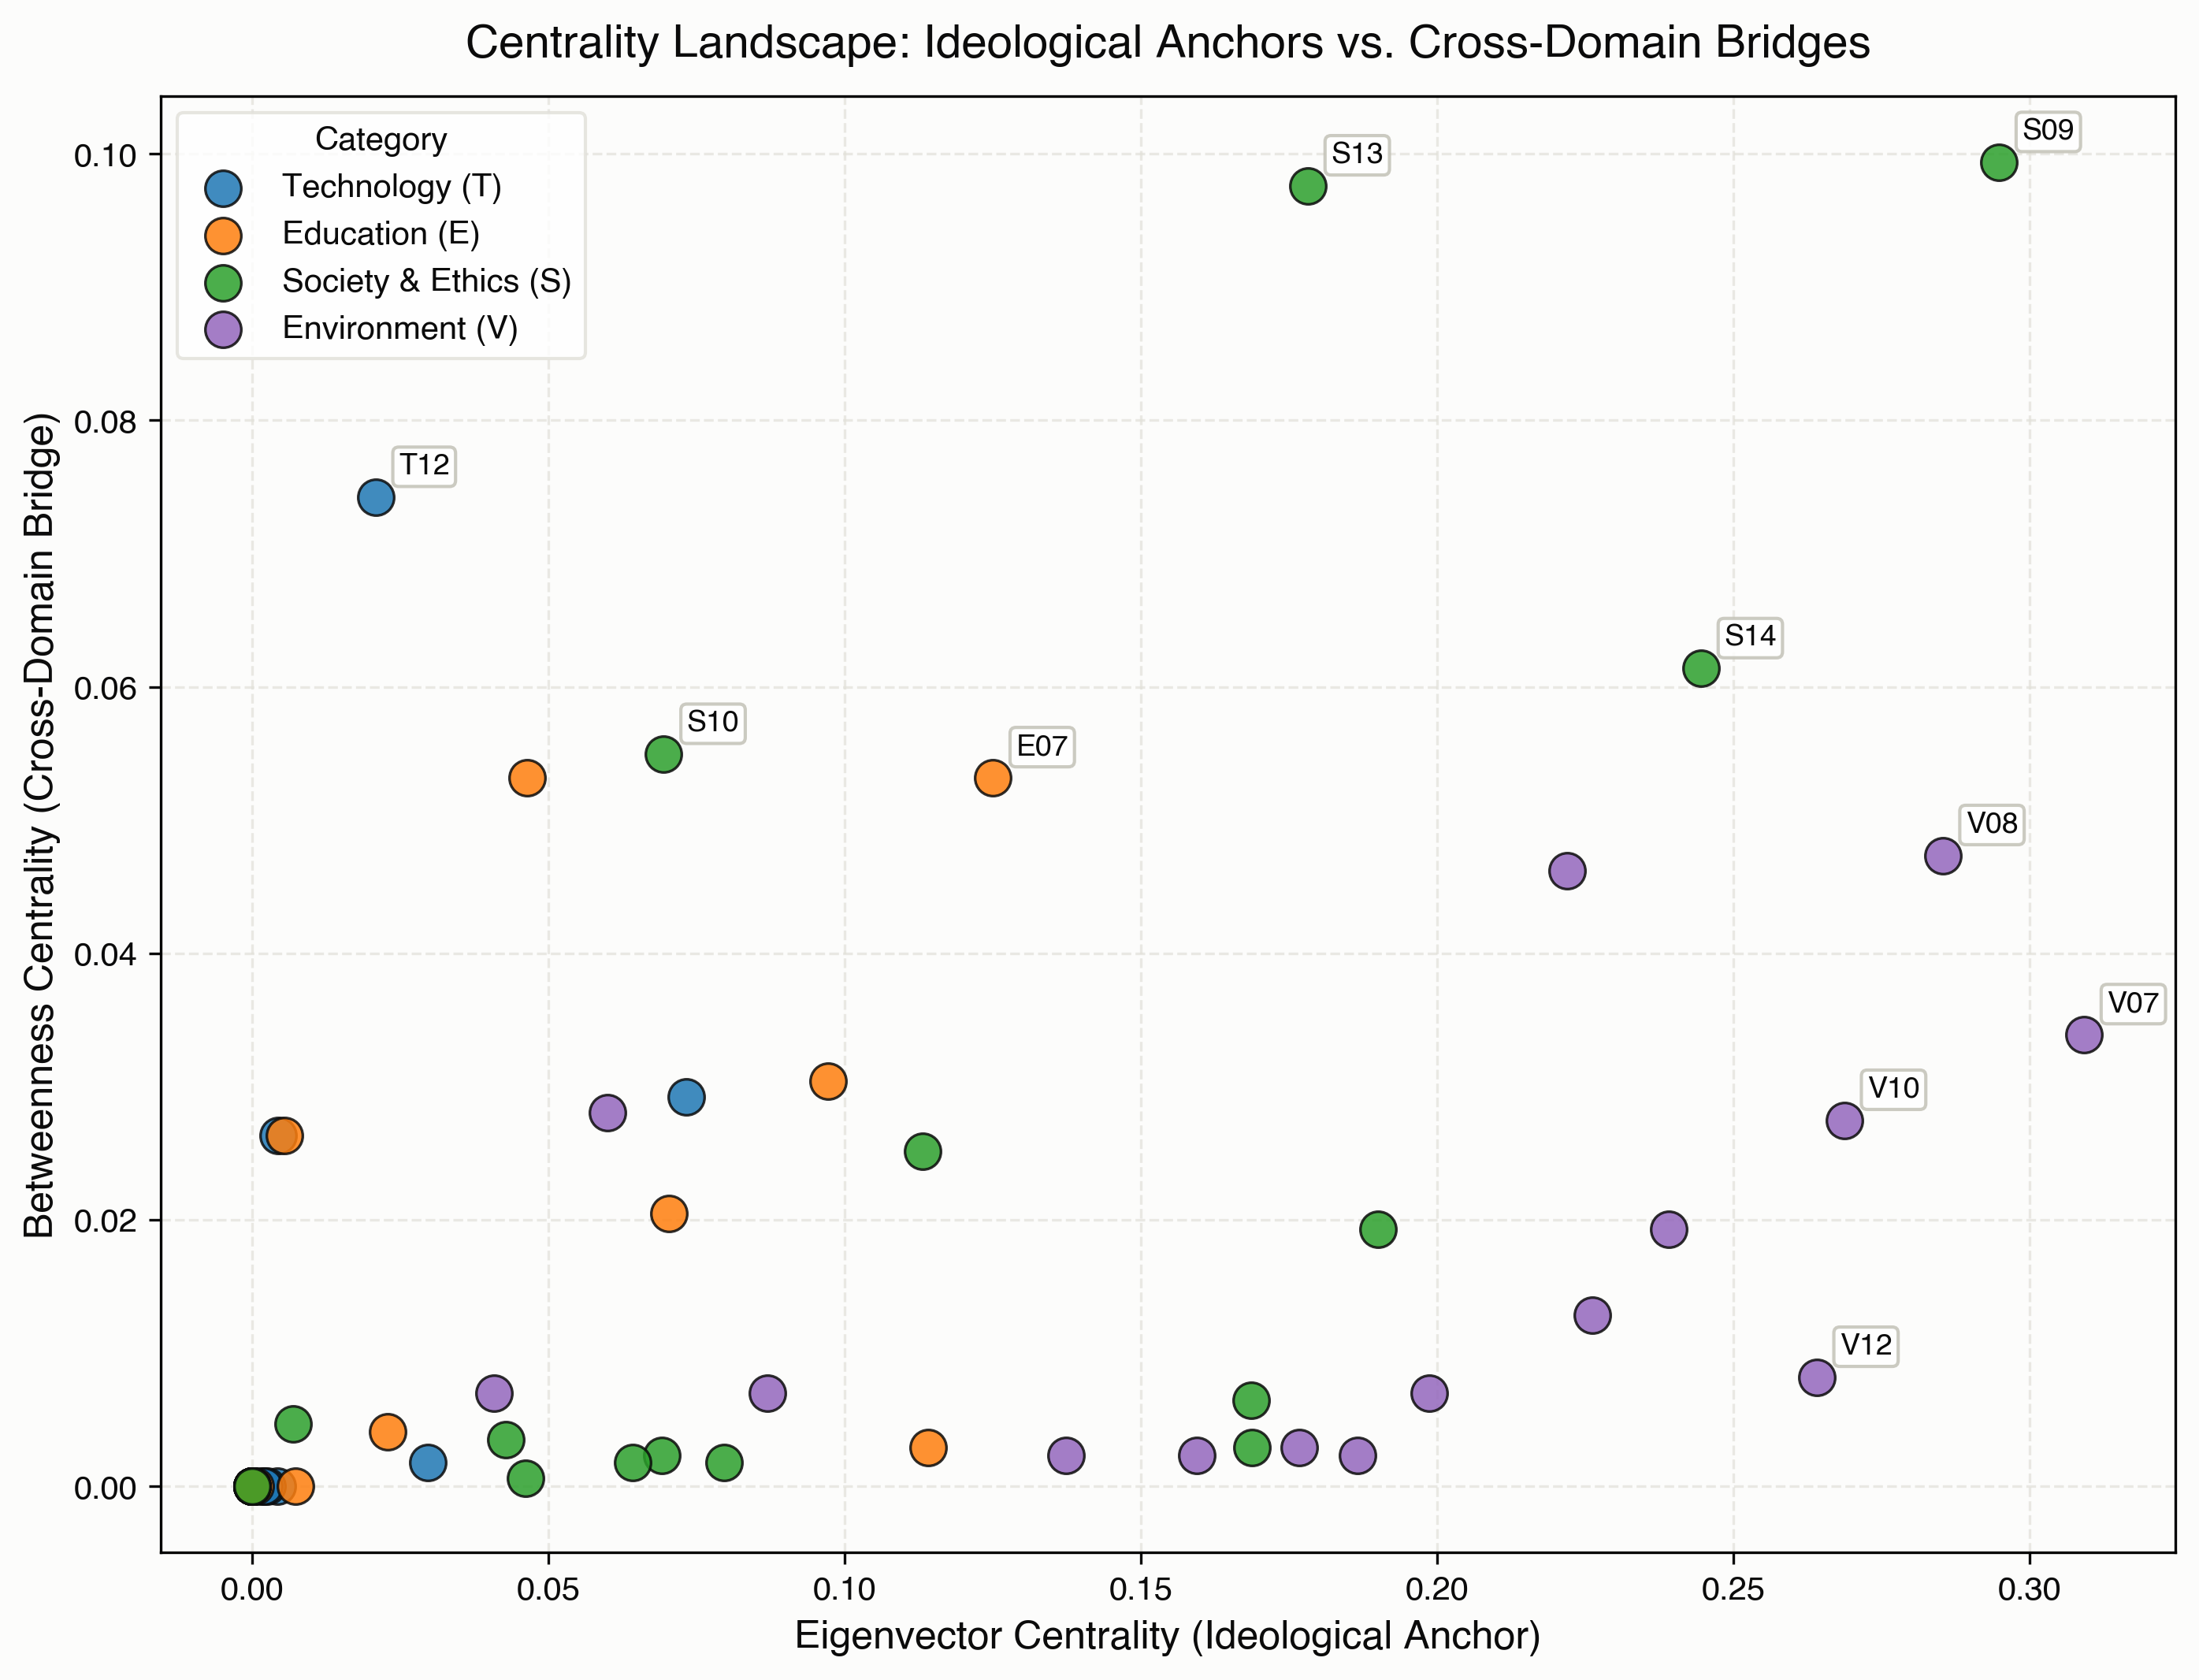
\includegraphics[width=0.48\textwidth]{Question Network/centrality_landscape.png}
    \caption{\textbf{Question Correlation Network and Centrality Landscape:} (Left) Spring layout with node size proportional to Eigenvector Centrality and colors representing predefined domains. (Right) Centrality Landscape: Eigenvector anchors vs. Betweenness bridges.}
    \label{fig:question_network_landscape}
\end{figure}

\begin{figure}[H]
    \centering
    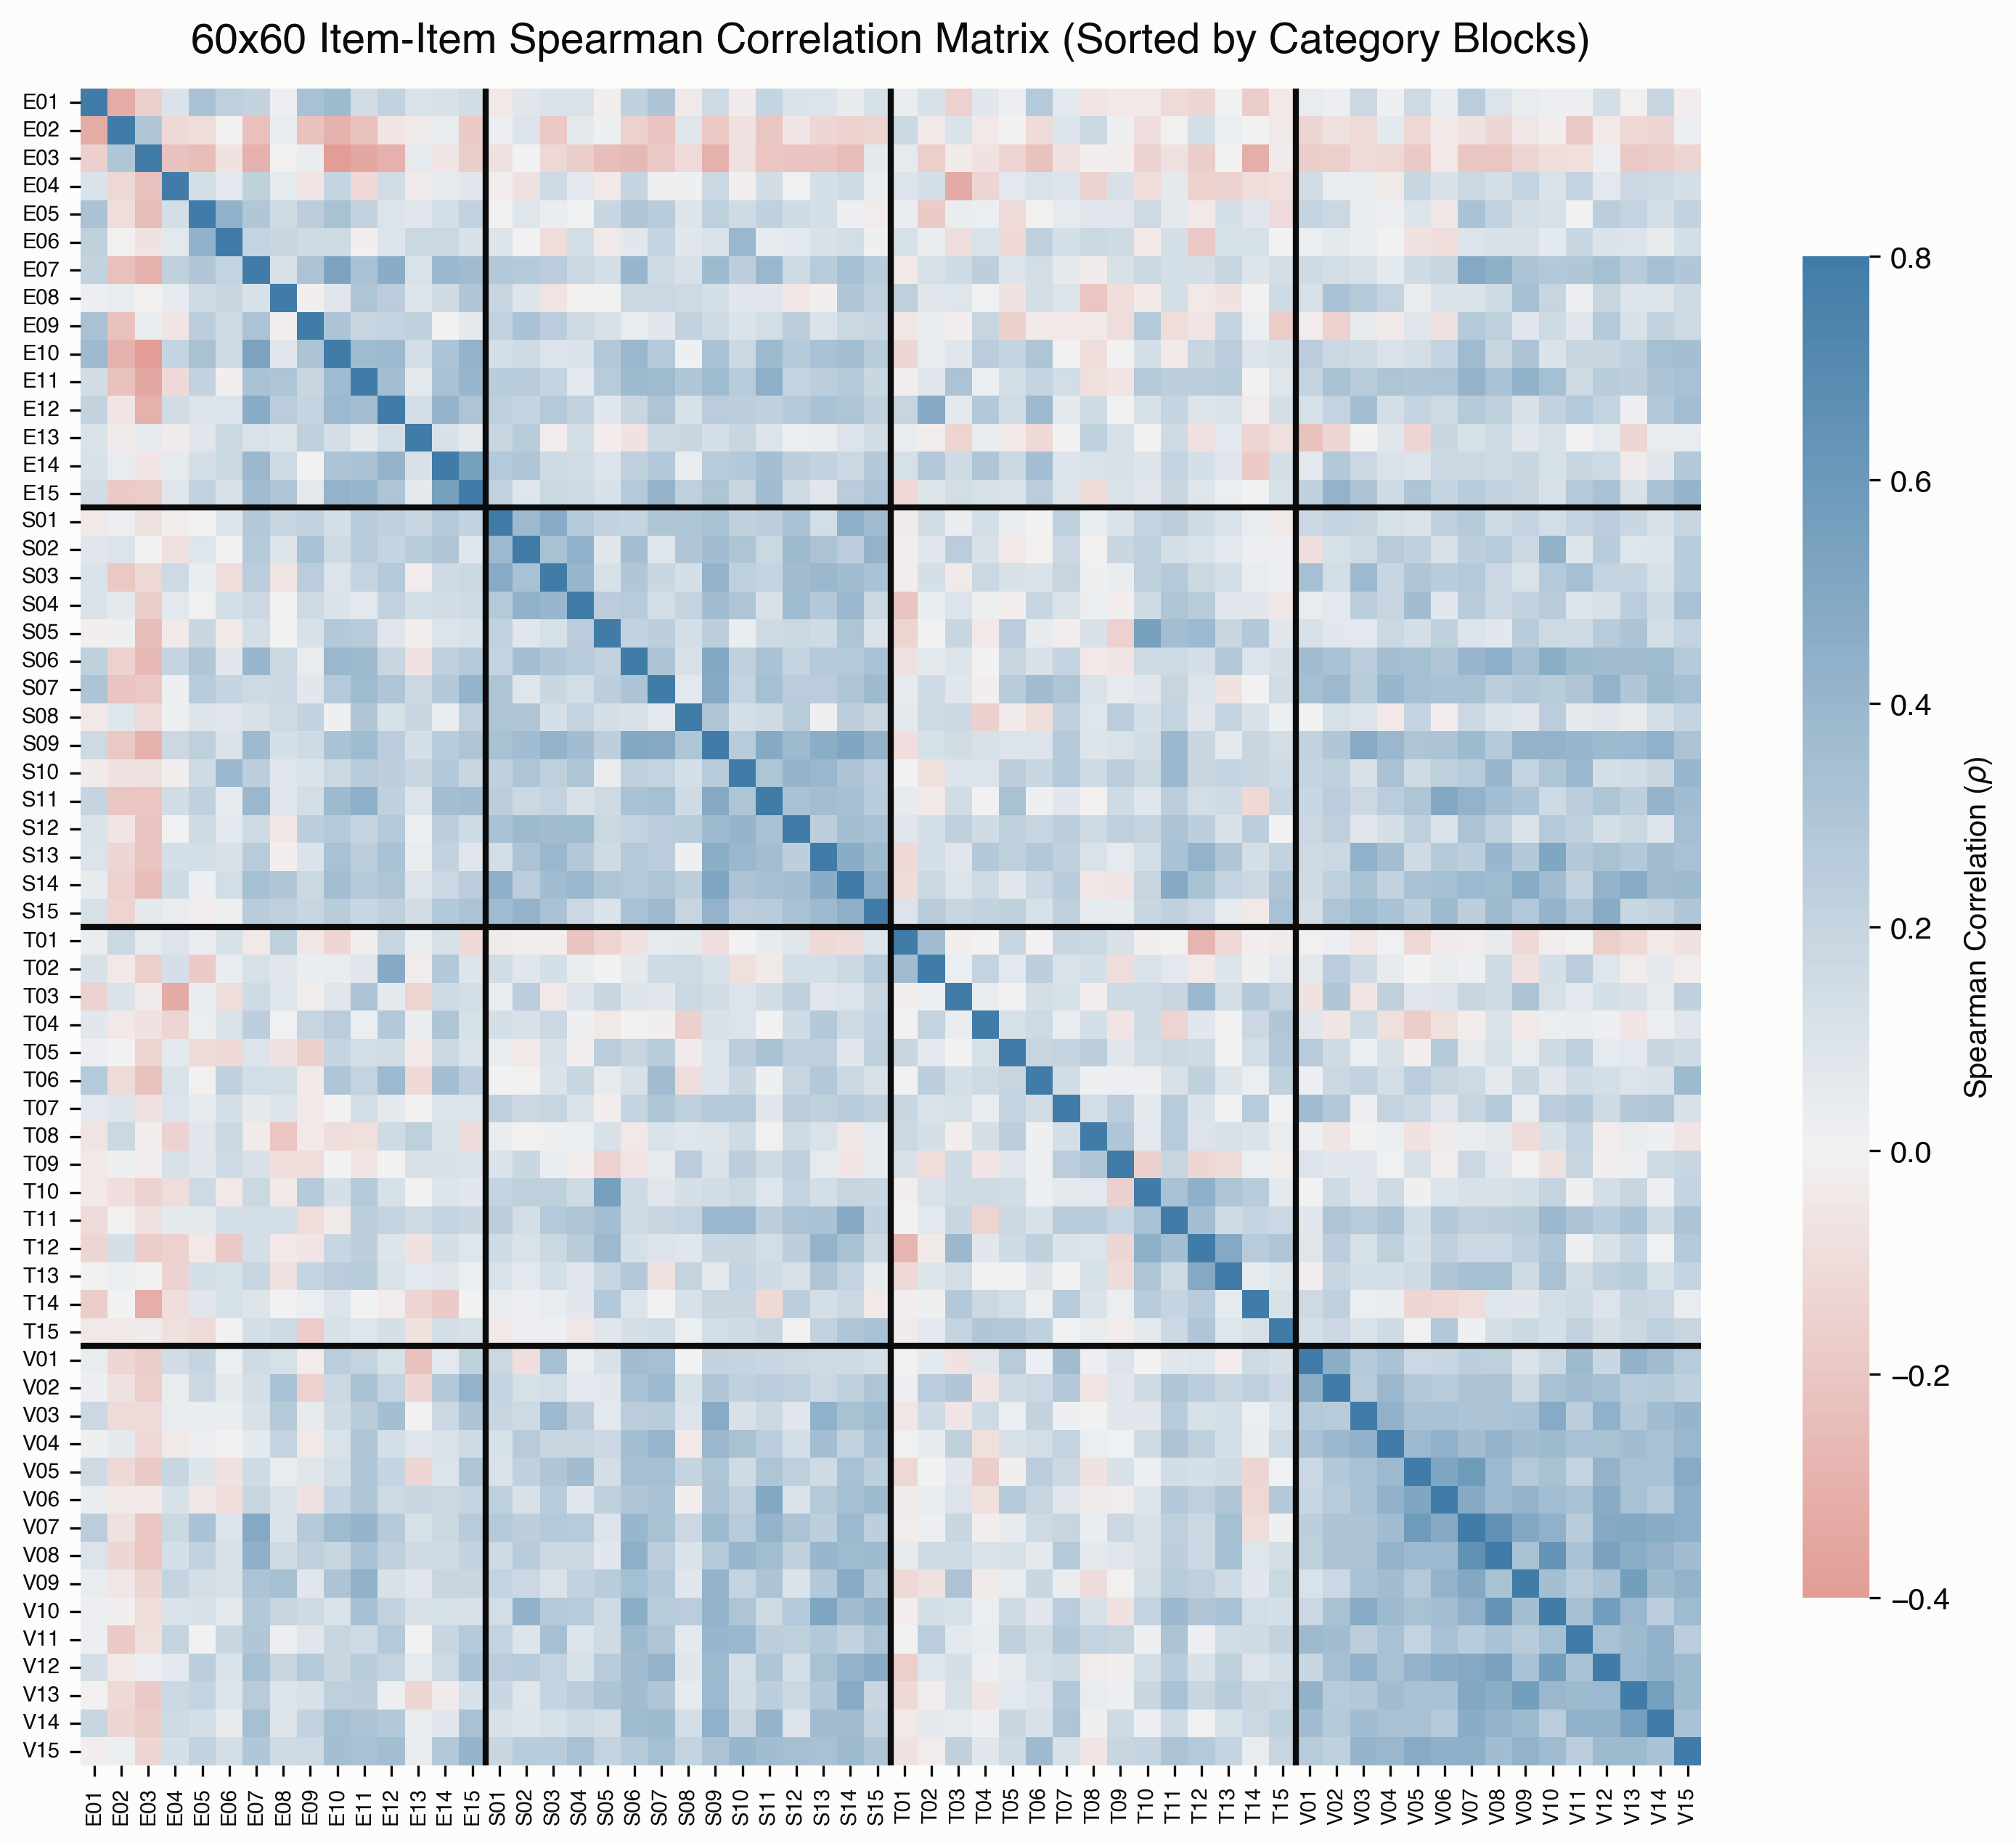
\includegraphics[width=0.48\textwidth]{Question Network/correlation_heatmap.png} \hfill
    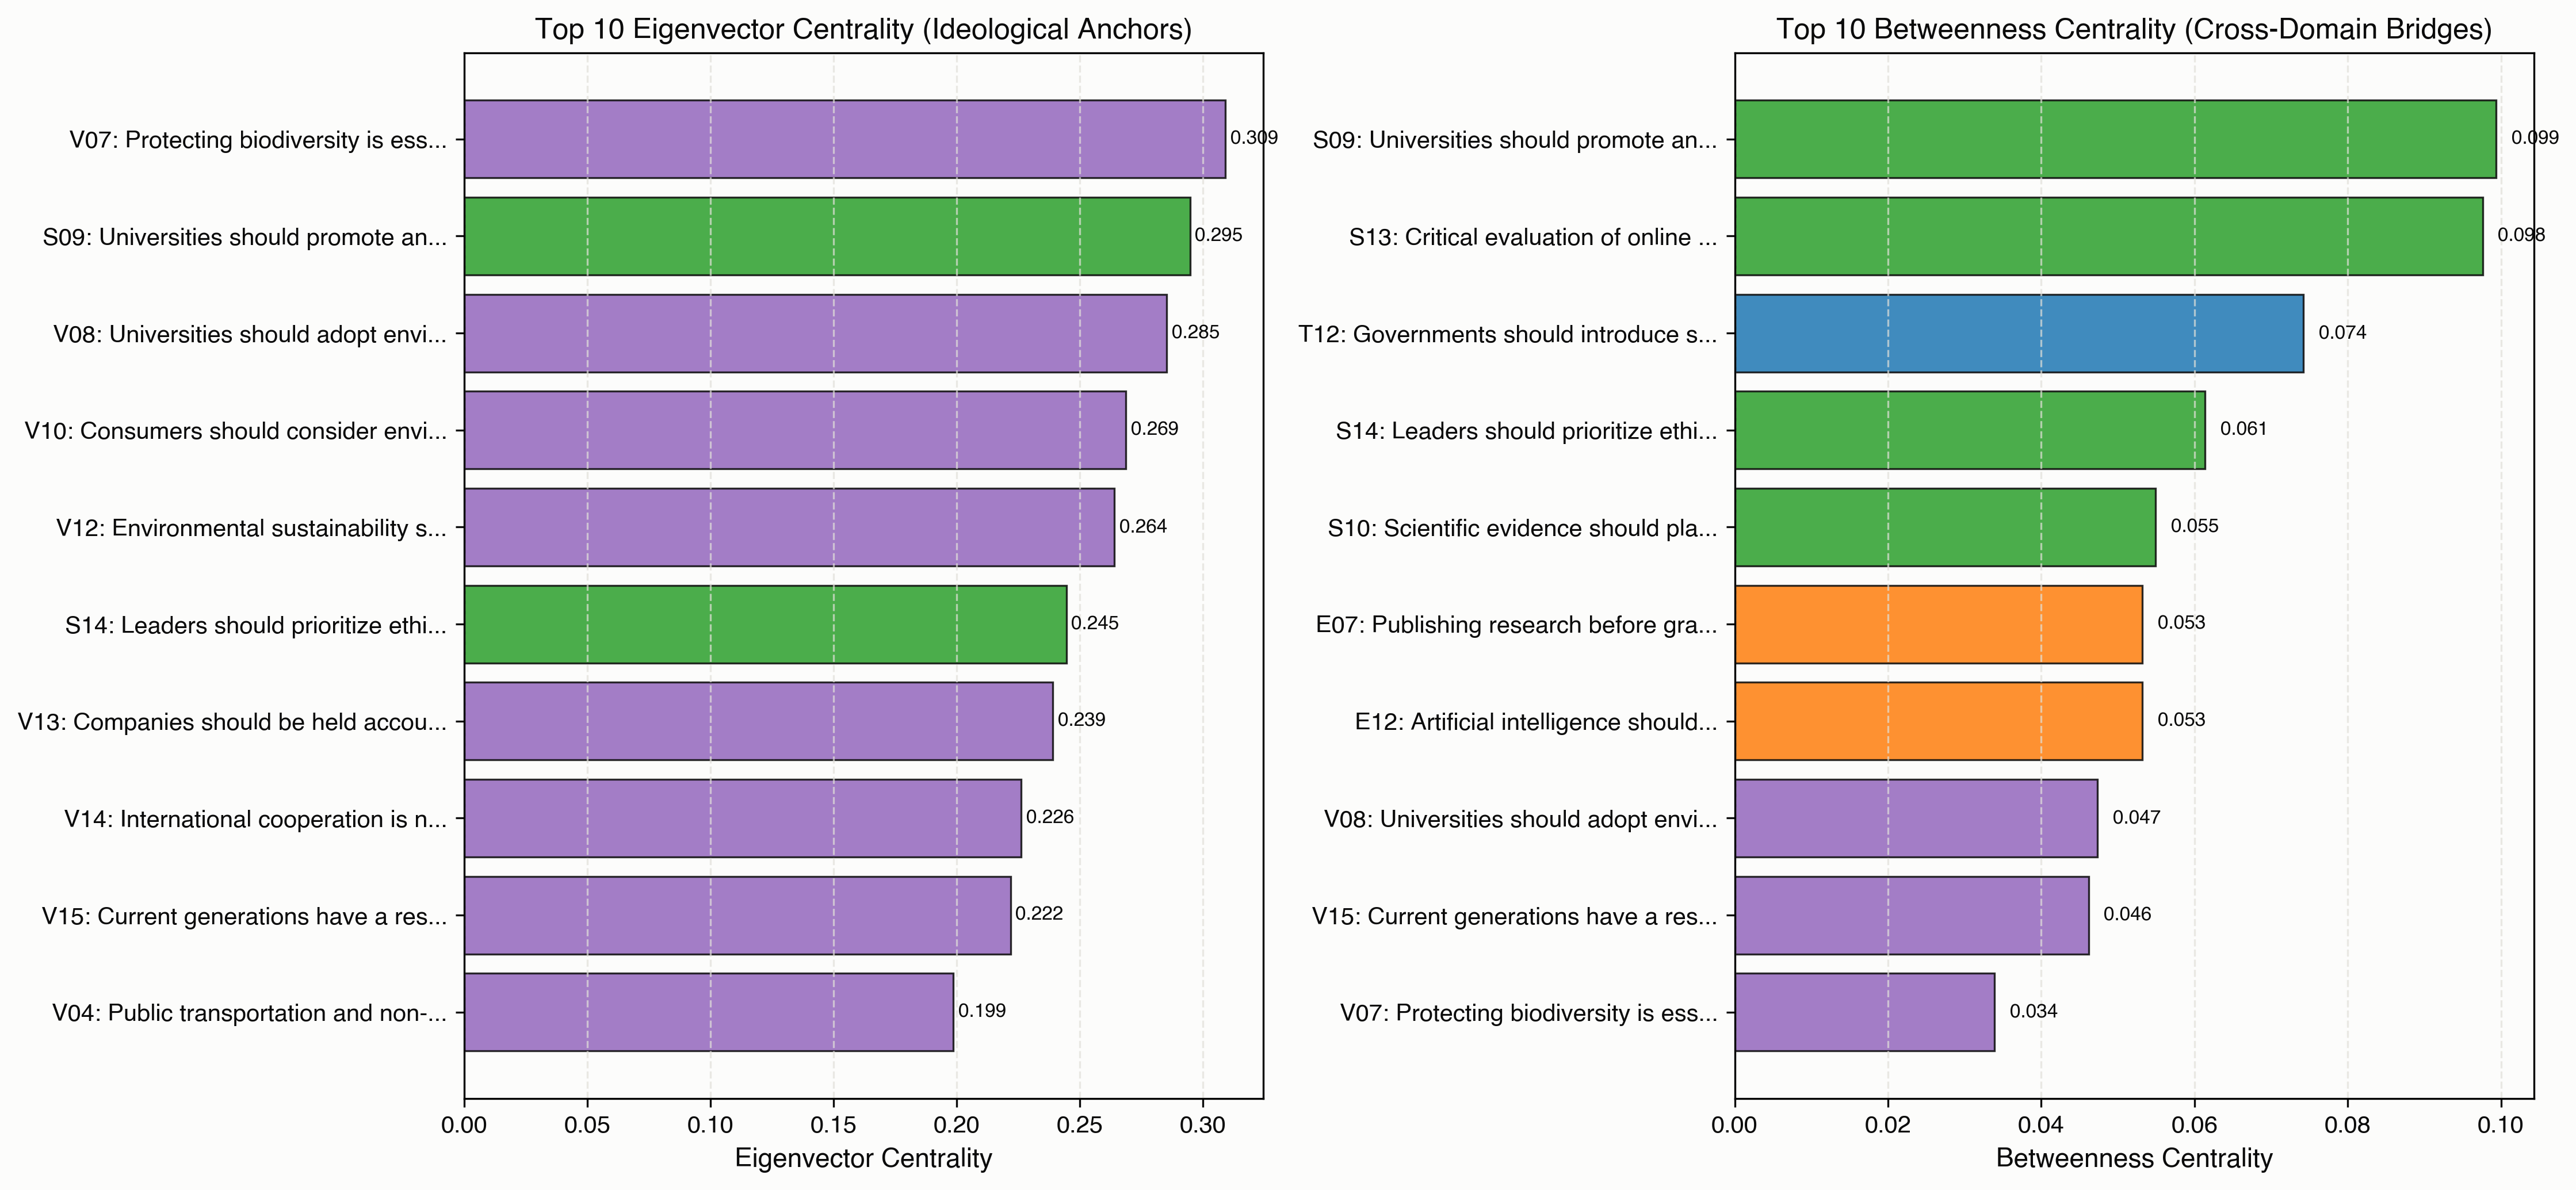
\includegraphics[width=0.48\textwidth]{Question Network/centrality_rankings.png}
    \caption{\textbf{Correlation Heatmap and Centrality Rankings:} (Left) 60$\times$60 Spearman matrix organized by category blocks. (Right) Top 10 rankings for Eigenvector (anchors) and Betweenness (bridges).}
    \label{fig:question_heatmap_rankings}
\end{figure}

\begin{table}[H]
\centering
\small
\caption{Top 5 Ideological Anchors (Eigenvector) and Top 5 Cross-Domain Bridges (Betweenness)}
\label{tab:item_centrality_table}
\begin{tabular}{llrrl}
\toprule
\textbf{Role} & \textbf{ID} & \textbf{Cat.} & \textbf{Score} & \textbf{Statement Excerpt} \\
\midrule
\textbf{Eigenvector Anchor}  & \texttt{V07} & V & 0.3092 & Protecting biodiversity is essential for long-term human welfare \\
                             & \texttt{S09} & S & 0.2948 & Universities should promote an inclusive environment for diversity \\
                             & \texttt{V08} & V & 0.2853 & Universities should adopt sustainable campus practices \\
                             & \texttt{V10} & V & 0.2687 & Consumers should consider environmental impact when purchasing \\
                             & \texttt{V12} & V & 0.2641 & Environmental sustainability should be integrated in higher ed \\
\midrule
\textbf{Betweenness Bridge}  & \texttt{S09} & S & 0.0994 & Universities should promote an inclusive environment for diversity \\
                             & \texttt{S13} & S & 0.0976 & Critical evaluation of online info must be taught as digital literacy \\
                             & \texttt{T12} & T & 0.0742 & Governments should introduce stricter regulations for AI development \\
                             & \texttt{S14} & S & 0.0614 & Leaders should prioritize ethics even when compromising short-term gains \\
                             & \texttt{S10} & S & 0.0549 & Scientific evidence should play an important role in public policy \\
\bottomrule
\end{tabular}
\end{table}

%% ====================================================================
\section{Results and Discussion: Decoding Class Beliefs and Ideological Dynamics}
%% ====================================================================

\subsection{The Ideological Core: Environmental and Institutional Consensus}
Eigenvector centrality identifies statements whose endorsement strongly co-occurs with endorsement of other highly central, influential propositions across the cohort. The empirical results yield a striking pattern: \textbf{8 of the top 10 eigenvector nodes belong to Category V (Environment)}, headed by \texttt{V07} (0.3092), \texttt{V08} (0.2853), \texttt{V10} (0.2687), \texttt{V12} (0.2641), and \texttt{V13} (0.2391), seamlessly integrated with universal institutional ethics statements \texttt{S09} (0.2948) and \texttt{S14} (0.2445).

\textbf{Substantive Interpretation:} Environmental stewardship and institutional ethics serve as the \textbf{unquestioned moral bedrock of the student population}. Rather than being contentious or marginal policy debates, ecological sustainability operates as a dense, mutually-reinforcing consensus module. Endorsement of biodiversity conservation (\texttt{V07}) or green campus operations (\texttt{V08}) is tightly coupled with broad support for corporate accountability (\texttt{V13}) and ethical governance (\texttt{S14}). In contrast to technological adoption or pedagogical grading models—where trade-offs provoke debate—students treat environmental responsibility and campus inclusivity not as negotiable choices, but as foundational prerequisites underpinning contemporary society.

\subsection{The Bridges: Cross-Disciplinary Synthesis and Pedagogical Levers}
Betweenness centrality isolates items controlling the shortest topological paths between otherwise separate thematic modules, identifying issues that function as \textbf{conceptual translators}:
\begin{itemize}
    \setlength{\itemsep}{0pt}
    \item \textbf{\texttt{S09} (Campus Diversity \& Inclusion, $b = 0.0994$):} Displays extraordinary dual centrality (Rank 1 in betweenness, Rank 2 in eigenvector). It acts as the master global bridge, connecting university pedagogical practices (\texttt{E}) to broader civic and environmental ethics (\texttt{S} and \texttt{V}).
    \item \textbf{\texttt{S13} (Critical Digital Literacy, $b = 0.0976$):} Sits squarely at the Technology--Education boundary, articulating that algorithmic information proliferation necessitates educational curricular reform.
    \item \textbf{\texttt{T12} (AI Regulation \& Governance, $b = 0.0742$):} Bridges pure technology items with public policy and legal safeguards, determining whether students view AI through an engineering or governance lens.
    \item \textbf{\texttt{E12} (AI as a Supportive Educational Tool, $b = 0.0532$):} Directly mediates between pedagogical philosophies and emerging technological adoption.
\end{itemize}

\textbf{Pedagogical \& Policy Implications:} Bridge items represent the highest-leverage intervention targets for policy and classroom discussion. While ideological anchors reinforce preexisting consensus, debates surrounding \texttt{T12}, \texttt{S13}, and \texttt{E12} possess the topological potential to cascade opinion shifts across multiple disciplinary domains.

\subsection{Organic Clustering vs. Predefined Categories}
The category attribute assortativity coefficient is $r = 0.3044$. While positive (confirming moderate within-category homophily), it is substantially lower than unity, demonstrating that \textbf{students do not organize their beliefs according to academic silos}. Louvain community detection partitions the network into six organic multi-item modules:
\begin{enumerate}
    \setlength{\itemsep}{0pt}
    \item \textbf{Module 1: AI Governance \& Algorithmic Safety (\texttt{T03}, \texttt{T10}, \texttt{T12}, \texttt{T13}, \texttt{S05}):} Technology is fused with regulatory safeguards, copyright disclosure, and data privacy.
    \item \textbf{Module 2: Academic Science \& Public Policy (\texttt{E05}, \texttt{E06}, \texttt{S10}):} Blends university research publishing norms with evidence-based governance.
    \item \textbf{Module 3: Educational Modernization \& EdTech (13 items):} Fuses higher education items (\texttt{E01}, \texttt{E07}, \texttt{E10}--\texttt{E12}, \texttt{E14}, \texttt{E15}) with foundational technology tools (\texttt{T01}, \texttt{T02}, \texttt{T06}) and ethical skills (\texttt{S07}, \texttt{S11}, \texttt{V02}).
    \item \textbf{Module 4: Civic Responsibility, Equity, \& Consumer Ethics (12 items):} Integrates human rights and diversity (\texttt{S01}--\texttt{S04}, \texttt{S09}, \texttt{S12}--\texttt{S15}) with ethical consumerism (\texttt{V03}, \texttt{V10}) and data privacy (\texttt{T11}).
    \item \textbf{Module 5: Pure Ecological Stewardship (8 items):} An unmixed environmental cluster (\texttt{V04}--\texttt{V09}, \texttt{V12}, \texttt{V15}) reflecting tight domain insularity around biodiversity and climate conservation.
    \item \textbf{Module 6: Global Infrastructure \& Corporate Accountability:} \texttt{V01}, \texttt{V11}, \texttt{V13}, \texttt{V14}, \texttt{T07}, \texttt{S06}.
\end{enumerate}
\textbf{The 13 Isolated Questions:} Items such as \texttt{T04}, \texttt{T08}, \texttt{E02}, \texttt{E08}, and \texttt{S08} failed to correlate with any item above $\rho > 0.35$. These correspond to specialized, divisive, or idiosyncratic prompts (e.g., radical techno-optimism or niche grading mechanics) that students evaluate independently of collective ideological packages.

\subsection{Triangulating the Class Mindset: A Multi-Model Synthesis}
Triangulating the three network paradigms yields a unified understanding of class opinion formation:
\begin{enumerate}
    \setlength{\itemsep}{0pt}
    \item \textbf{Absence of Echo Chambers:} The student network exhibits smooth degradation under sparsification; the bipartite projection is complete ($K_{60}$ with $\kappa = 59.0 \gg 2$); and the item correlation graph maintains a robust 47-node giant component. The cohort displays zero tribal polarization or ideological fragmentation.
    \item \textbf{Passion vs. Agreement:} While the student network captures broad agreement, the bipartite network identifies where passion is concentrated: the Keystone Trio (\texttt{E15}, \texttt{E11}, \texttt{V13}) draws extreme conviction from over 67\% of students.
    \item \textbf{Domain Independence:} Society and Environment align closely across students ($r = 0.46$), while Technology and Education operate independently ($r = 0.16$), confirming that technological optimism does not dictate pedagogical philosophy.
\end{enumerate}

\subsection{What the Networks Reveal About Class Opinions}
Synthesizing our empirical results across the three analytical lenses reveals several profound insights into the collective psychology and socio-technical mindset of this student cohort:
\begin{itemize}
    \setlength{\itemsep}{1pt}
    \item \textbf{Ecological Stewardship as Non-Negotiable Civic Ethos:} Environmental concerns (\texttt{V07}, \texttt{V08}, \texttt{V10}, \texttt{V12}) dominate both the eigenvector core in the correlation network and the highest passion degrees in the bipartite network. Unlike contested policy debates, ecological preservation and sustainable campus standards serve as universally endorsed baseline values that bridge students across divergent academic tracks.
    \item \textbf{Pragmatic Technocentrism vs. Unchecked Optimism:} While the cohort demonstrates strong enthusiasm for experiential tech tools and AI in education (\texttt{E11}, \texttt{E12}), it simultaneously displays critical awareness of algorithmic harms. By tightly coupling AI regulation (\texttt{T12}) and digital literacy (\texttt{S13}) as pivotal geodesic bridges, students indicate that technological adoption must be circumscribed by rigorous ethical oversight and democratic accountability.
    \item \textbf{Absence of Polarization and Fragmented Subcultures:} Neither the chance-adjusted student network nor the bipartite conviction graph displays structural balkanization. Even under strict filtering for extreme views ($\tau \in \{1, 5\}$), the projected network forms a complete clique $K_{60}$ with a Molloy--Reed parameter of $\kappa = 59.0 \gg 2$, confirming that ideological diversity in this cohort manifests as nuanced variations in emphasis rather than entrenched partisan antagonism.
    \item \textbf{Pedagogical Modernization Demands:} In education, students heavily cluster around statements favoring practical, experiential curriculum redesign and collaborative AI utilization over rigid traditional rote assessments. This aligns with modern pedagogical paradigms advocating for active learning and transparent academic governance.
\end{itemize}

\subsection{Methodological Implications and Web Portal Hosting}
By decoupling ambient positivity from structural association, our tri-partite methodology demonstrates that real-world opinion mining requires multiple complementary network representations: \textit{Student projections} measure interpersonal consensus and cohesion; \textit{Bipartite extreme filtering} isolates ideological intensity and percolation resilience; and \textit{Item correlations} uncover latent cognitive ontologies and structural bridges. To facilitate open scientific reproducibility and dynamic exploration, all 300~DPI high-resolution graphical representations, interactive D3.js force-directed graphs, and full question catalogs are permanently hosted on our public web dashboard at \url{https://your-username.github.io/DPCN_ass1/}.

%% ====================================================================
\section{Individual Contributions}
%% ====================================================================

\begin{table}[H]
\centering
\small
\begin{tabular}{p{2.6cm} p{4.6cm} p{8.8cm}}
\toprule
\textbf{Team Member} & \textbf{Network Domain} & \textbf{Specific Tasks Completed} \\
\midrule
\textbf{Mayank Kar} & Student--Student Network & Formulated chance-adjusted agreement metric, implemented sparsification threshold sweep, calculated small-world clustering/path metrics, and analyzed cross-topic concordance heatmaps. \\
\midrule
\textbf{Tanush Garg} & Question--Student Bipartite Network & Executed extreme conviction filtering ($\tau \in \{1, 5\}$), conducted linear/log-log degree distribution fitting, evaluated Molloy--Reed percolation, and generated bipartite projection graphs. \\
\midrule
\textbf{Amish Goyal} & Question--Question Network & Computed pairwise Spearman rank correlations ($\rho > 0.35$), evaluated weighted Eigenvector anchors and Betweenness bridges, ran Louvain community detection, assortativity, and compiled the synthesized report. \\
\bottomrule
\end{tabular}
\end{table}

\end{document}
